\chapter{Results}
This chapter presents all the results for the algorithms and computations mentioned in the previous chapters. As a brief reminder, the \emph{paraphrased} setting operates with samples from the datasets $\si \in D$ and $\spi \in D_p$ (see Equation~\ref{eq:paraphrasing}) while the \emph{model-generated} setting operates with samples from the dataset $\si \in D$ and $\smi \in D_m$ (see Equation~\ref{eq:model_generated_sample}. Concretely, the evaluation checks whether flattened gradients $\vXspi[\theta]$ (paraphrased) and $\vXsmi[\theta]$ (model-generated) retrieve their corresponding original samples $\vXsi[\theta]$ via cosine similarity, following Equation~\ref{eq:cosine_similarity_paraphrased} and the accuracy metric defined in Equation~\ref{eq:accuracy_bm25}.
\\\\
The remainder of the chapter is organized as follows. Section~\ref{sec:baseline_perf} reports baseline retrieval results using the full model gradient. Section~\ref{sec:single_layer_perf} analyzes contributions per component. Section~\ref{sec:layer_vs_full} compares single-component scores to full-model scores. Section~\ref{sec:greedy_vs_rp} evaluates compact surrogates via forward greedy selection against a random-projection baseline. Section~\ref{sec:exec_time} summarizes the cost profile.

\section{Performance of Gradient Similarity as an Explanation Method}\label{sec:baseline_perf}
All gradient similarities are computed and reconstructed from stored dot products using Equations~\ref{eq:dot_grad_decompose} to represent the cosine similarities for both the paraphrased ($\simcos(\vXspi, \vXsj)$) and the model-generated ($\simcos(\vXsmi, \vXsj)$) case, $\forall \spi \in D_p$ and $\forall \smi \in D_m$. To avoid the comparison of all-pairs $\mathcal{O}(N^2)$, for each paraphrased (or model-generated) sample $\sj \in \mathcal{C}_i(b)$ is restricted to a BM25 candidate set with $b=5$ (Algorithm~\ref{alg:bm25_select_samples}). The metrics $\operatorname{accuracy}^{(b)}_{\theta}(D_p,D)$ and $\operatorname{accuracy}^{(b)}_{\theta}(D_m,D)$ are then evaluated as in Equation~\ref{eq:accuracy_bm25}.
\begin{table}[h]
    \centering
    \begin{tabular}{|l|c|c|}
        \hline
        \textbf{Model} & \textbf{Paraphrased} & \textbf{Model-generated} \\
        \hline
        AMD-OLMo-1B-SFT & 0.993 & 0.218 \\
        \hline
    \end{tabular}
    \caption{Score for $\operatorname{accuracy}^{(b)}_{\theta}(D_p,D)$ (paraphrased) and $\operatorname{accuracy}^{(b)}_{\theta}(D_m,D)$ (model-generated) cases with the full model gradient.}
    \label{tab:model_accuracy}
\end{table}
As shown in Table~\ref{tab:model_accuracy}, the gradient similarity method is able to find nearly all original samples when queried with the paraphrased samples of $D_p$. For the model-generated setting, this is very different, as it can only identify approximately one out of five original samples when queried with the dataset $D_m$. When considering that random guessing would lead to a baseline of $0.2$ due to the candidate set having a size of $\lvert\mathcal{C}_i(b)\rvert = 5$ since $b=5$ and $1 \div 5=0.2$, the accuracy is not far off.
\\\\
In the paraphrased setting, only seven samples are wrongly assigned to their original counterparts. It seems that they are not wrongly assigned by coincidence, they are connected by some patterns. For example, three of them (with the ids lima\_725, lima\_767 and lima\_773) have very long assistant messages resulting in token sequences with more than $2950$ items, despite \texttt{AMD-OLMo-1B-SFT} only having a context size of $2048$. 
\fxnote{Illustrate similarities between samples that have been classified wrongly and give a short example}

\section{Single Layer Performance}\label{sec:single_layer_perf}
This section quantifies the contribution of \emph{single} layer components to retrieval and similarity. For each parameter matrix $\Wlk$, the BM25-restricted retrieval accuracy $\operatorname{accuracy}^{(b)}_{\Wlk}(\cdot,D)$ (Equation~\ref{eq:layer_accuracy_bm25}) is evaluated to test whether the gradient of a \emph{single} component suffices to recover the original sample. All quantities are reconstructed from per-component dot products (Section~\ref{subsec:intermediate_results}), so no full gradients are materialized.
\\\\
The results are reported for both settings (\textbf{paraphrased} and \textbf{model-generated}), aggregated across depth and component family (Embedding; Attention $Q/K/V/O$; MLP gate/up/down). The medians across layers are shown for robustness against outliers (Table~\ref{tab:average_accuracy_layer_component}), and depth-wise trends are visualized in Figures~\ref{fig:paraphrased_accuracy_per_layer}~and~\ref{fig:model_generated_accuracy_per_layer}.
\begin{table}[H]
    \centering
    \begin{tabular}{|c|c|c|c|}
        \hline
        & \textbf{Layer Component} & \textbf{Paraphrased} & \textbf{Model-generated} \\
        \hline
        \multirow{1}{5em}{Embedding}
        & Embedding & 0.993 & 0.231 \\
        \hline
        \multirow{4}{5em}{Attention}
        & Query-Projection & 0.979 & 0.253 \\
        & Key-Projection & 0.916 & 0.211 \\
        & Value-Projection & 0.982 & 0.188 \\
        & Output-Projection & 0.994 & 0.205 \\
        \hline
        \multirow{3}{5em}{MLP}
        & Gate-Projection & 0.994 & 0.265 \\
        & Up-Projection & 0.993 & 0.26 \\
        & Down-Projection & 0.995 & 0.221 \\
        \hline
    \end{tabular}
    \caption{Averaged (median) layer component accuracy for the paraphrased ($\operatorname{accuracy}^{(b)}_{\Wlk}(D_p,D)$) and the model-generated ($\operatorname{accuracy}^{(b)}_{\Wlk}(D_m,D)$) case.}
    \label{tab:average_accuracy_layer_component}
\end{table}
\noindent As shown in Table~\ref{tab:average_accuracy_layer_component}, single-component gradients already suffice to recover the original item in the \emph{paraphrased} setting: median accuracies exceed $0.98$ for all components except the key projection ($0.916$), with the MLP path (gate/up/down) and the attention output projection matching or slightly surpassing the full-model score ($\approx 0.99$). This indicates that paraphrasing preserves gradient directions consistently across layers, so gradients from individual components contain enough information to identify the correct original sample. In contrast, the \emph{model-generated} setting collapses toward the $0.2$ random-guess baseline level imposed by $b{=}5$: accuracies cluster near baseline, with only the MLP (gate/up at $\approx 0.26$) and the query projection ($0.253$) providing a small, repeatable improvement; the value projection falls below baseline ($0.188$). The embedding matrix reaches $0.231$, suggesting that lexical overlap alone is insufficient once responses are re-synthesized (model-generated). Overall, the information that supports correct retrieval is broadly distributed in the paraphrased condition but becomes concentrated mainly in the MLP and $Q$ projections in the model-generated condition, while $K$ and $V$ contribute the least to this retrieval objective.

\subsection{Does Size Matter?}
Here, \emph{size} refers to the number of parameters in a component ($4{,}194{,}304$ for the attention projections $Q/K/V/O$,
$16{,}777{,}216$ for the MLP projections gate/up/down, and $103{,}022{,}592$ for the embedding). Figure~\ref{fig:accuracy_per_layer_boxplot} summarizes retrieval accuracy for these three bins; the sub-panels
(Figs.~\ref{fig:accuracy_per_layer_boxplot_paraphrased}~and~\ref{fig:accuracy_per_layer_boxplot_model_generated}) correspond to the \emph{paraphrased} and \emph{model-generated} settings, respectively.
\\\\
In the \emph{paraphrased} condition (Fig.~\ref{fig:accuracy_per_layer_boxplot_paraphrased}), accuracies are essentially at ceiling across all sizes. The $4{,}194{,}304$ group exhibits a wider spread with several low outliers, whereas the $16{,}777{,}216$ group is tightly clustered near $0.99$ and the $103{,}022{,}592$ point (embedding) is at $0.993$. These differences are small. Because cosine similarity normalizes the vector magnitudes, the slight improvement observed for larger components is best interpreted as reduced variance rather than a substantive size effect.
\\\\
In the \emph{model-generated} condition
(Fig.~\ref{fig:accuracy_per_layer_boxplot_model_generated}), all groups concentrate a little bit above the $0.2$ random-guess baseline imposed by $b{=}5$. The $16{,}777{,}216$ group attains a marginally higher median ($\approx 0.24$–$0.25$) than the $4{,}194{,}304$ group ($\approx 0.21$–$0.23$), and the embedding ($103{,}022{,}592$) sits at $\approx 0.23$. Dispersion is largest for the $4{,}194{,}304$ group, which bundles both relatively stronger (e.g., $Q$) and weaker (e.g., $V$) projections despite identical size. This pattern indicates that \emph{component type}, not parameter count, drives the modest differences: MLP projections outperform on average, whereas $K$/$V$ lag, even though all four attention projections share the same size.
\\\\
Overall, there is no meaningful monotonic relationship between parameter count and retrieval accuracy. In the paraphrased setting, performance is uniformly high regardless of size; in the model-generated setting, accuracy hovers near baseline with only slight advantages for MLP-sized components. The functional role of a component within the architecture matters more than how many parameters it contains.
\begin{figure}[H]
    \centering
    \begin{subfigure}[h]{0.495\textwidth}
        \centering
        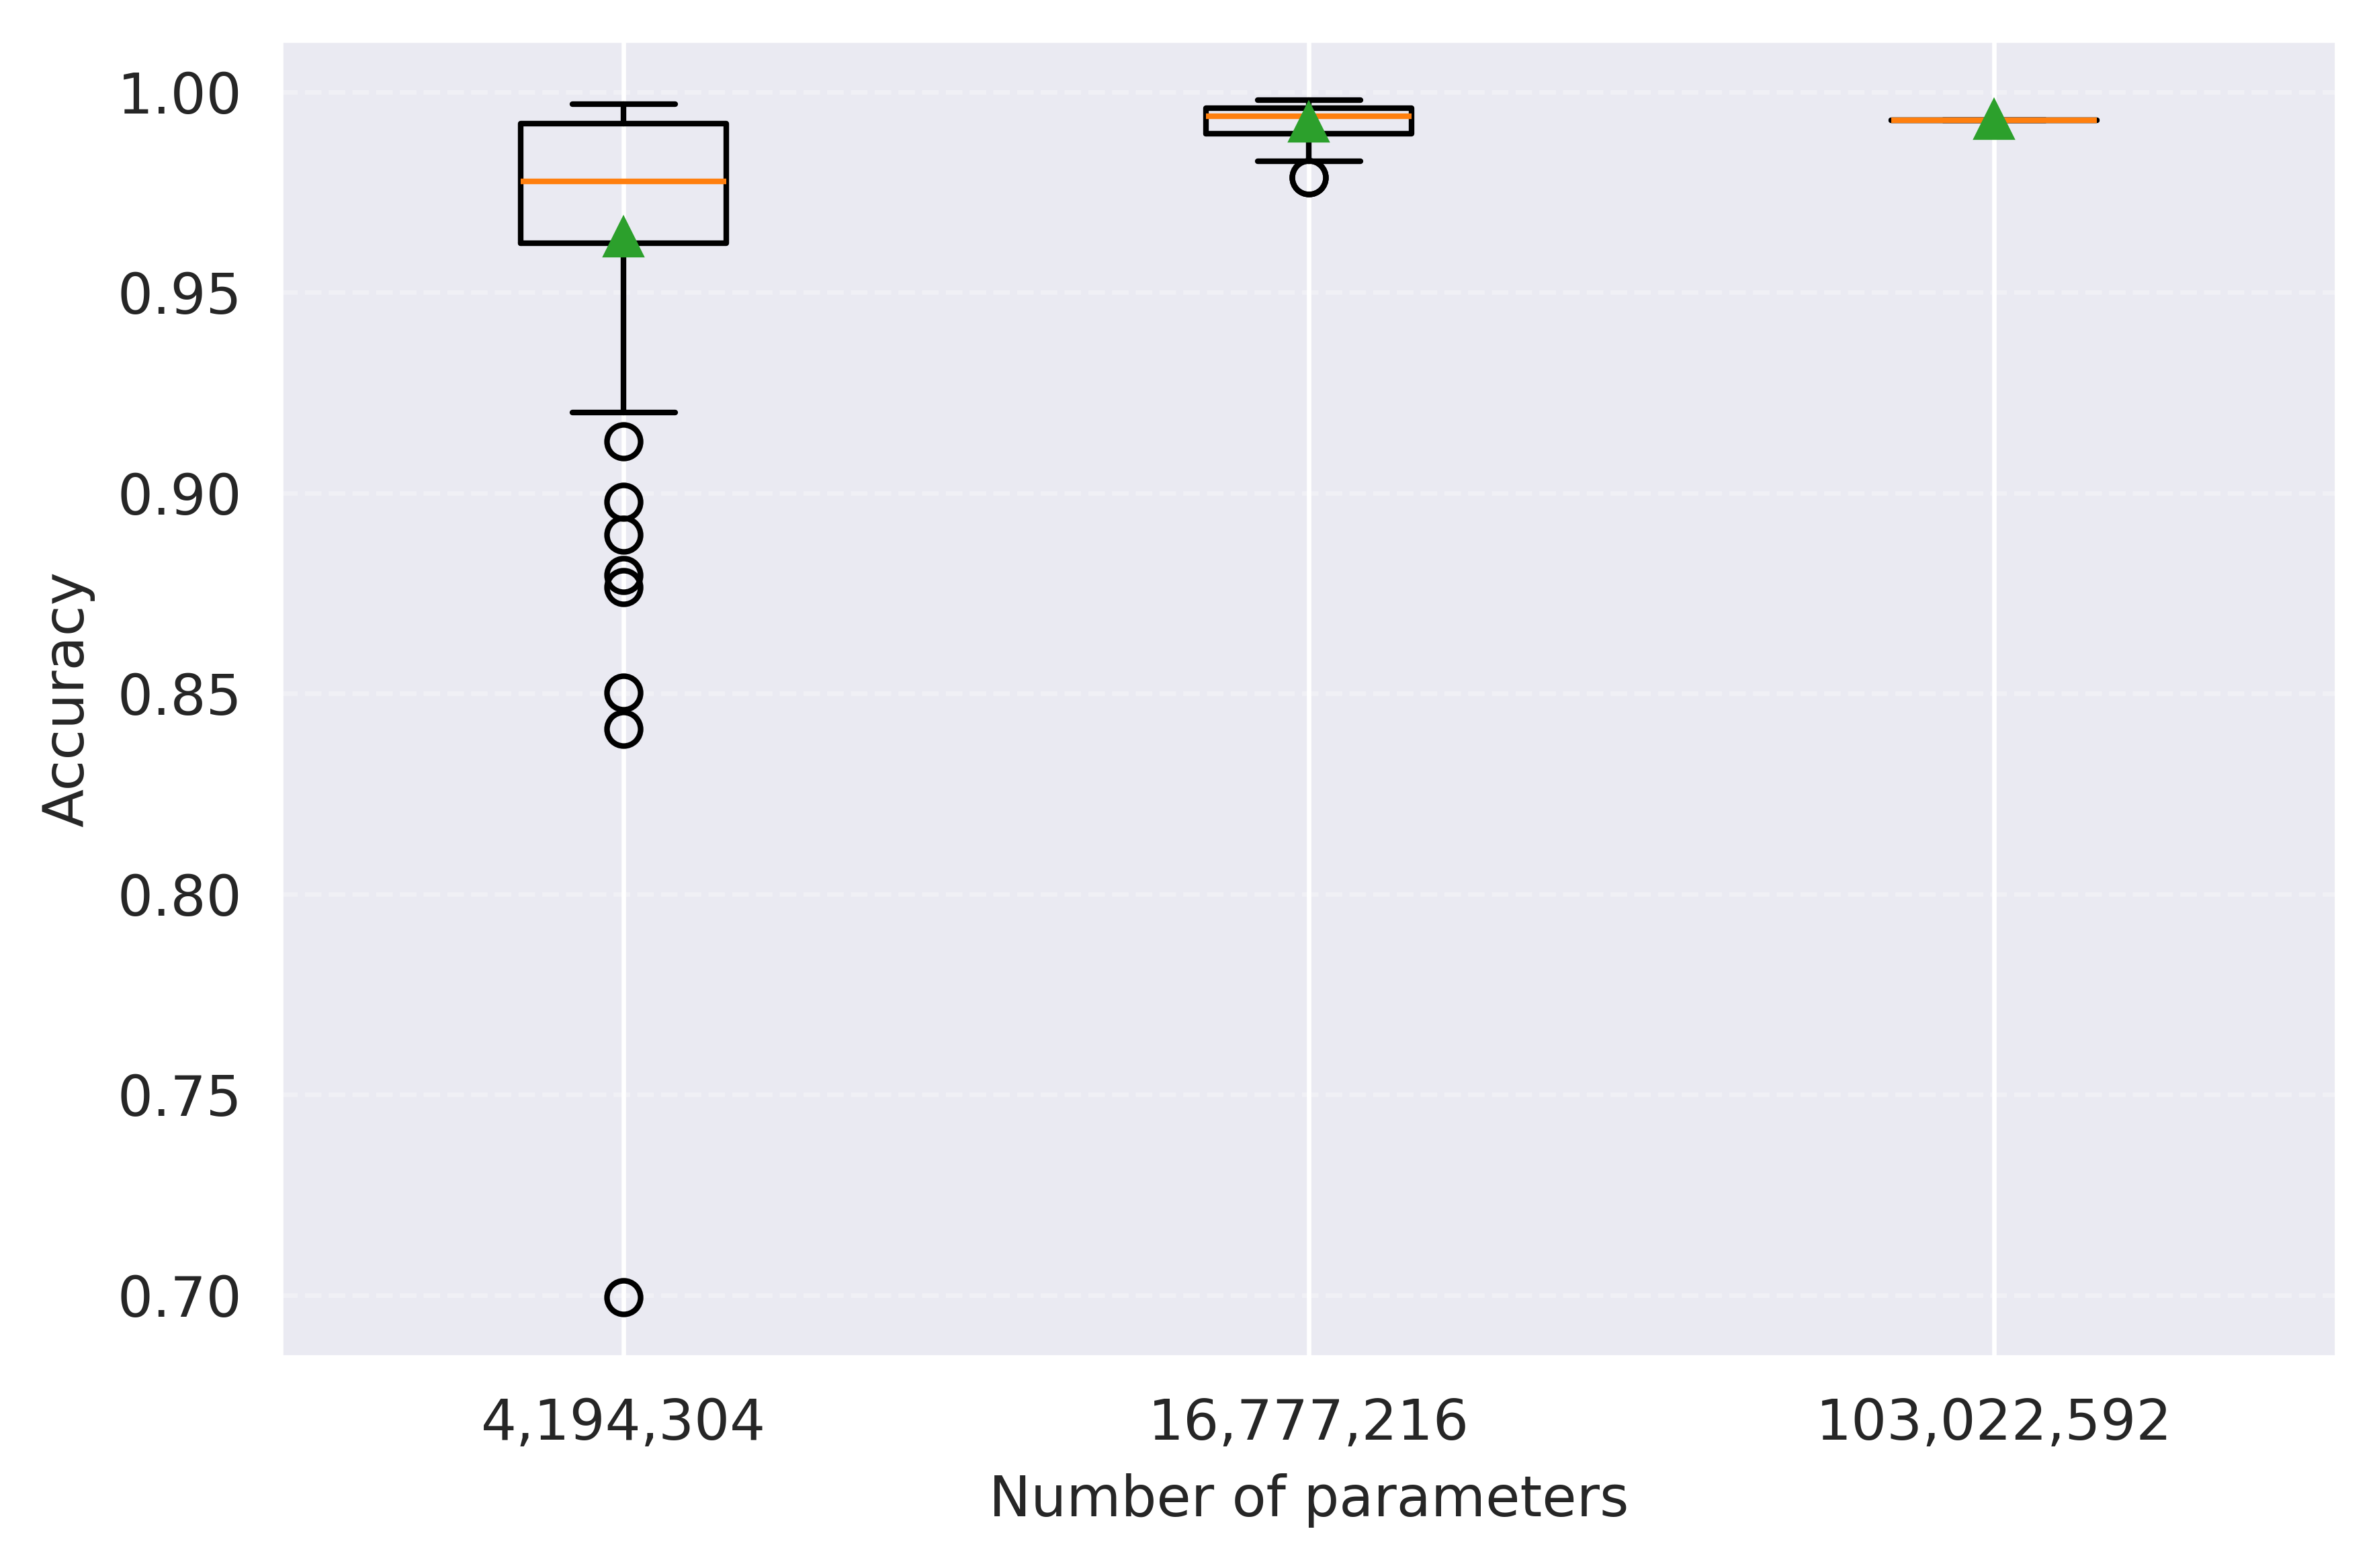
\includegraphics[width=\textwidth]{figures/results/paraphrased/accuracy_per_layer_boxplot.png}
        \caption{Paraphrased}
        \label{fig:accuracy_per_layer_boxplot_paraphrased}
    \end{subfigure}
    \hfill
    \begin{subfigure}[h]{0.495\textwidth}
        \centering
        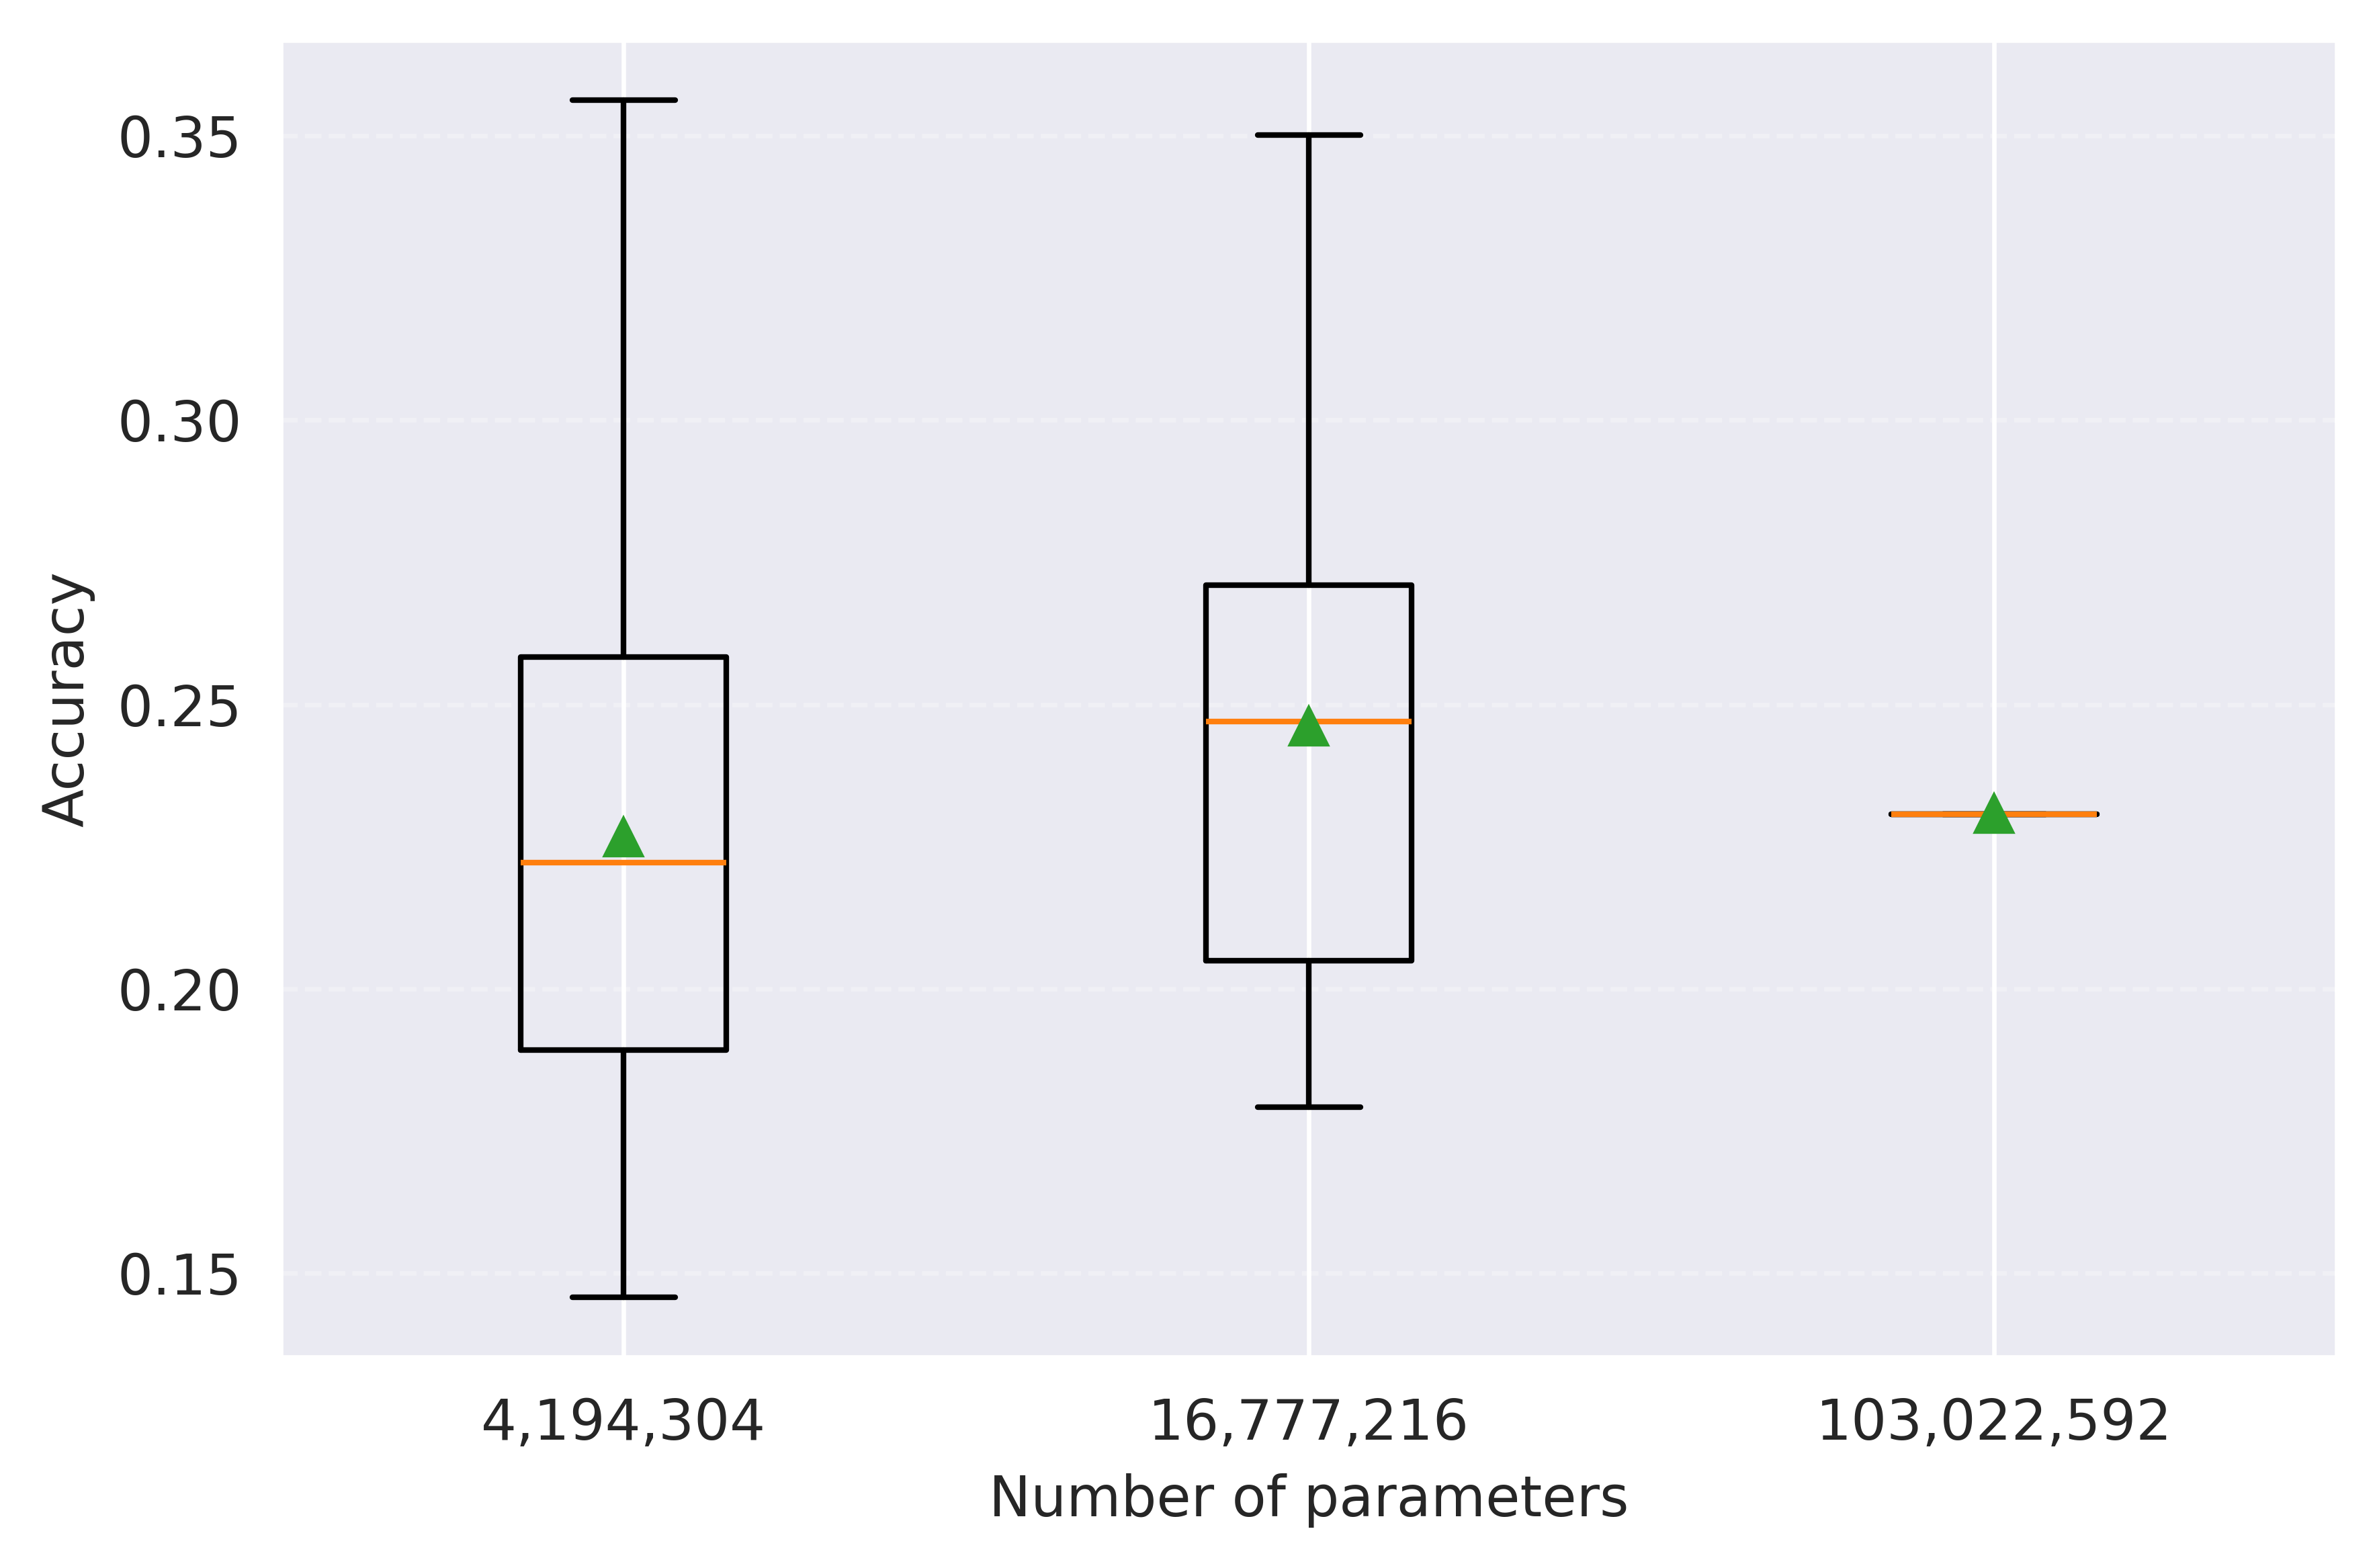
\includegraphics[width=\textwidth]{figures/results/model-generated/accuracy_per_layer_boxplot.png}
        \caption{Model-generated}
        \label{fig:accuracy_per_layer_boxplot_model_generated}
    \end{subfigure}
    \caption{Boxplots of layer component accuracy with respect to the number of parameters.}
    \label{fig:accuracy_per_layer_boxplot}
\end{figure}

\subsection{Does Depth Matter?}
Figure~\ref{fig:accuracy_over_layer_depth} reports the retrieval accuracy over layer depth ($l=0,\ldots,15$) when matching paraphrased/model-generated samples to their originals using gradient–cosine similarity within the BM25 candidate sets ($b{=}5$). Panels~\ref{fig:accuracy_over_layer_depth_attention_vs_mlp_paraphrased}~and~\ref{fig:accuracy_over_layer_depth_attention_vs_mlp_model_generated} aggregate over sub-components (Attention vs. MLP), while panels~\ref{fig:accuracy_over_layer_depth_attention_paraphrased}~-~\ref{fig:accuracy_over_layer_depth_mlp_model_generated} shows the accuracy for Attention $(Q/K/V/O)$ and MLP $(\text{gate}/\text{up}/\text{down})$.
\\\\
In the \emph{paraphrased} condition (left column), accuracies are near ceiling ($\approx0.95$–$1.00$) across most depths and components. MLP slightly but consistently outperforms Attention when averaged over sub-components (panel~\ref{fig:accuracy_over_layer_depth_attention_vs_mlp_paraphrased}). Within Attention (panel~\ref{fig:accuracy_over_layer_depth_attention_paraphrased}), $K$ is the weakest across depth and a pronounced drop for $V$ appears in the final layer, whereas $Q$ and $O$ remain close to the overall plateau. The trend with depth is monotone-increasing into upper layers with a shallow saturation at $\approx1.0$.
\\\\
In the \emph{model-generated} condition (right column), accuracies are substantially lower ($\approx0.18$–$0.33$), i.e., only modestly above the random baseline $1/b=0.20$. Performance is highest in early layers, dips in the middle, and recovers slightly toward the later layers (panel~\ref{fig:accuracy_over_layer_depth_attention_vs_mlp_model_generated}). MLP sub-components (panel~\ref{fig:accuracy_over_layer_depth_mlp_model_generated}) dominate Attention overall, and within Attention (panel~d) the ordering $Q,O > K,V$ is consistent across depth, with $V$ typically the weakest.
\\\\
Taken together, paraphrasing preserves gradient directions broadly—single components already suffice to retrieve the original—whereas model-regenerated outputs weaken alignment, concentrating useful signal in MLP and the $Q/O$ projections while $K/V$ contribute least to this retrieval objective.
\begin{figure}[htb]
    \centering
    \begin{subfigure}[h]{0.49\textwidth}
        \centering
        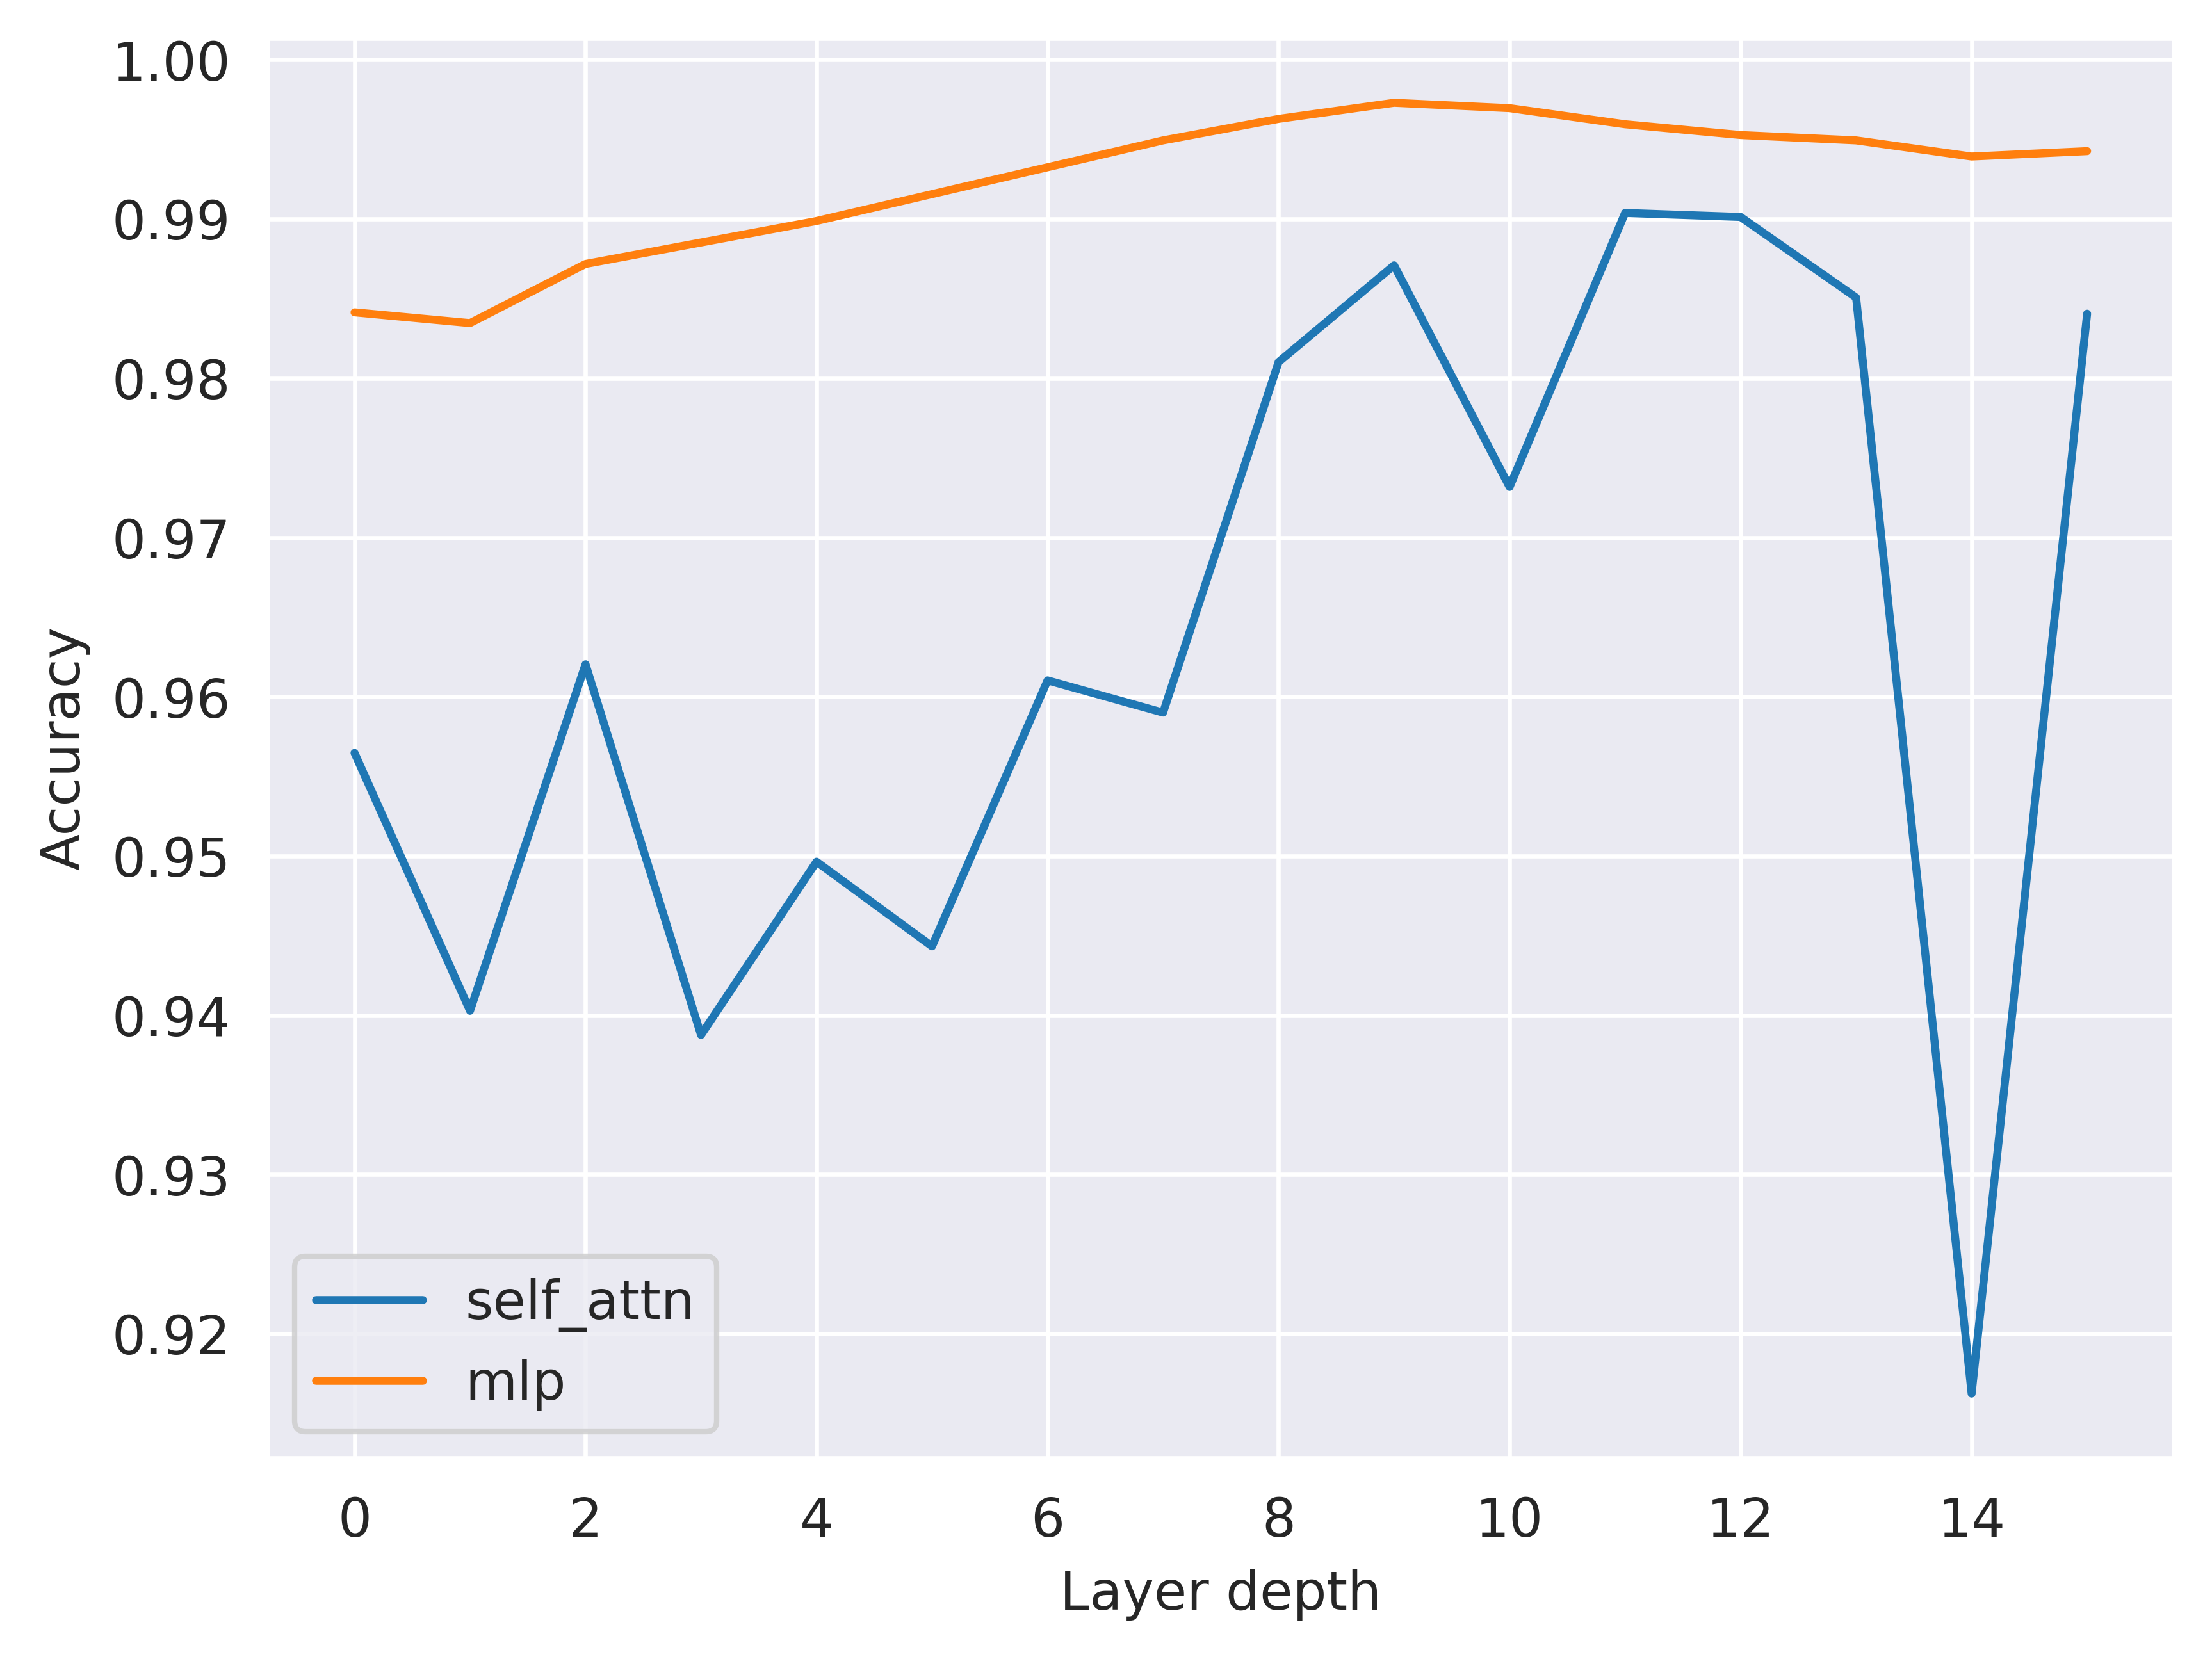
\includegraphics[width=\textwidth]{figures/results/paraphrased/overall_attention_vs_mlp.png}
        \caption{Mean accuracy: Attention vs. MLP (paraphrased).}                 % (a)
        \label{fig:accuracy_over_layer_depth_attention_vs_mlp_paraphrased}
    \end{subfigure}
    \hfill
    \begin{subfigure}[h]{0.49\textwidth}
        \centering
        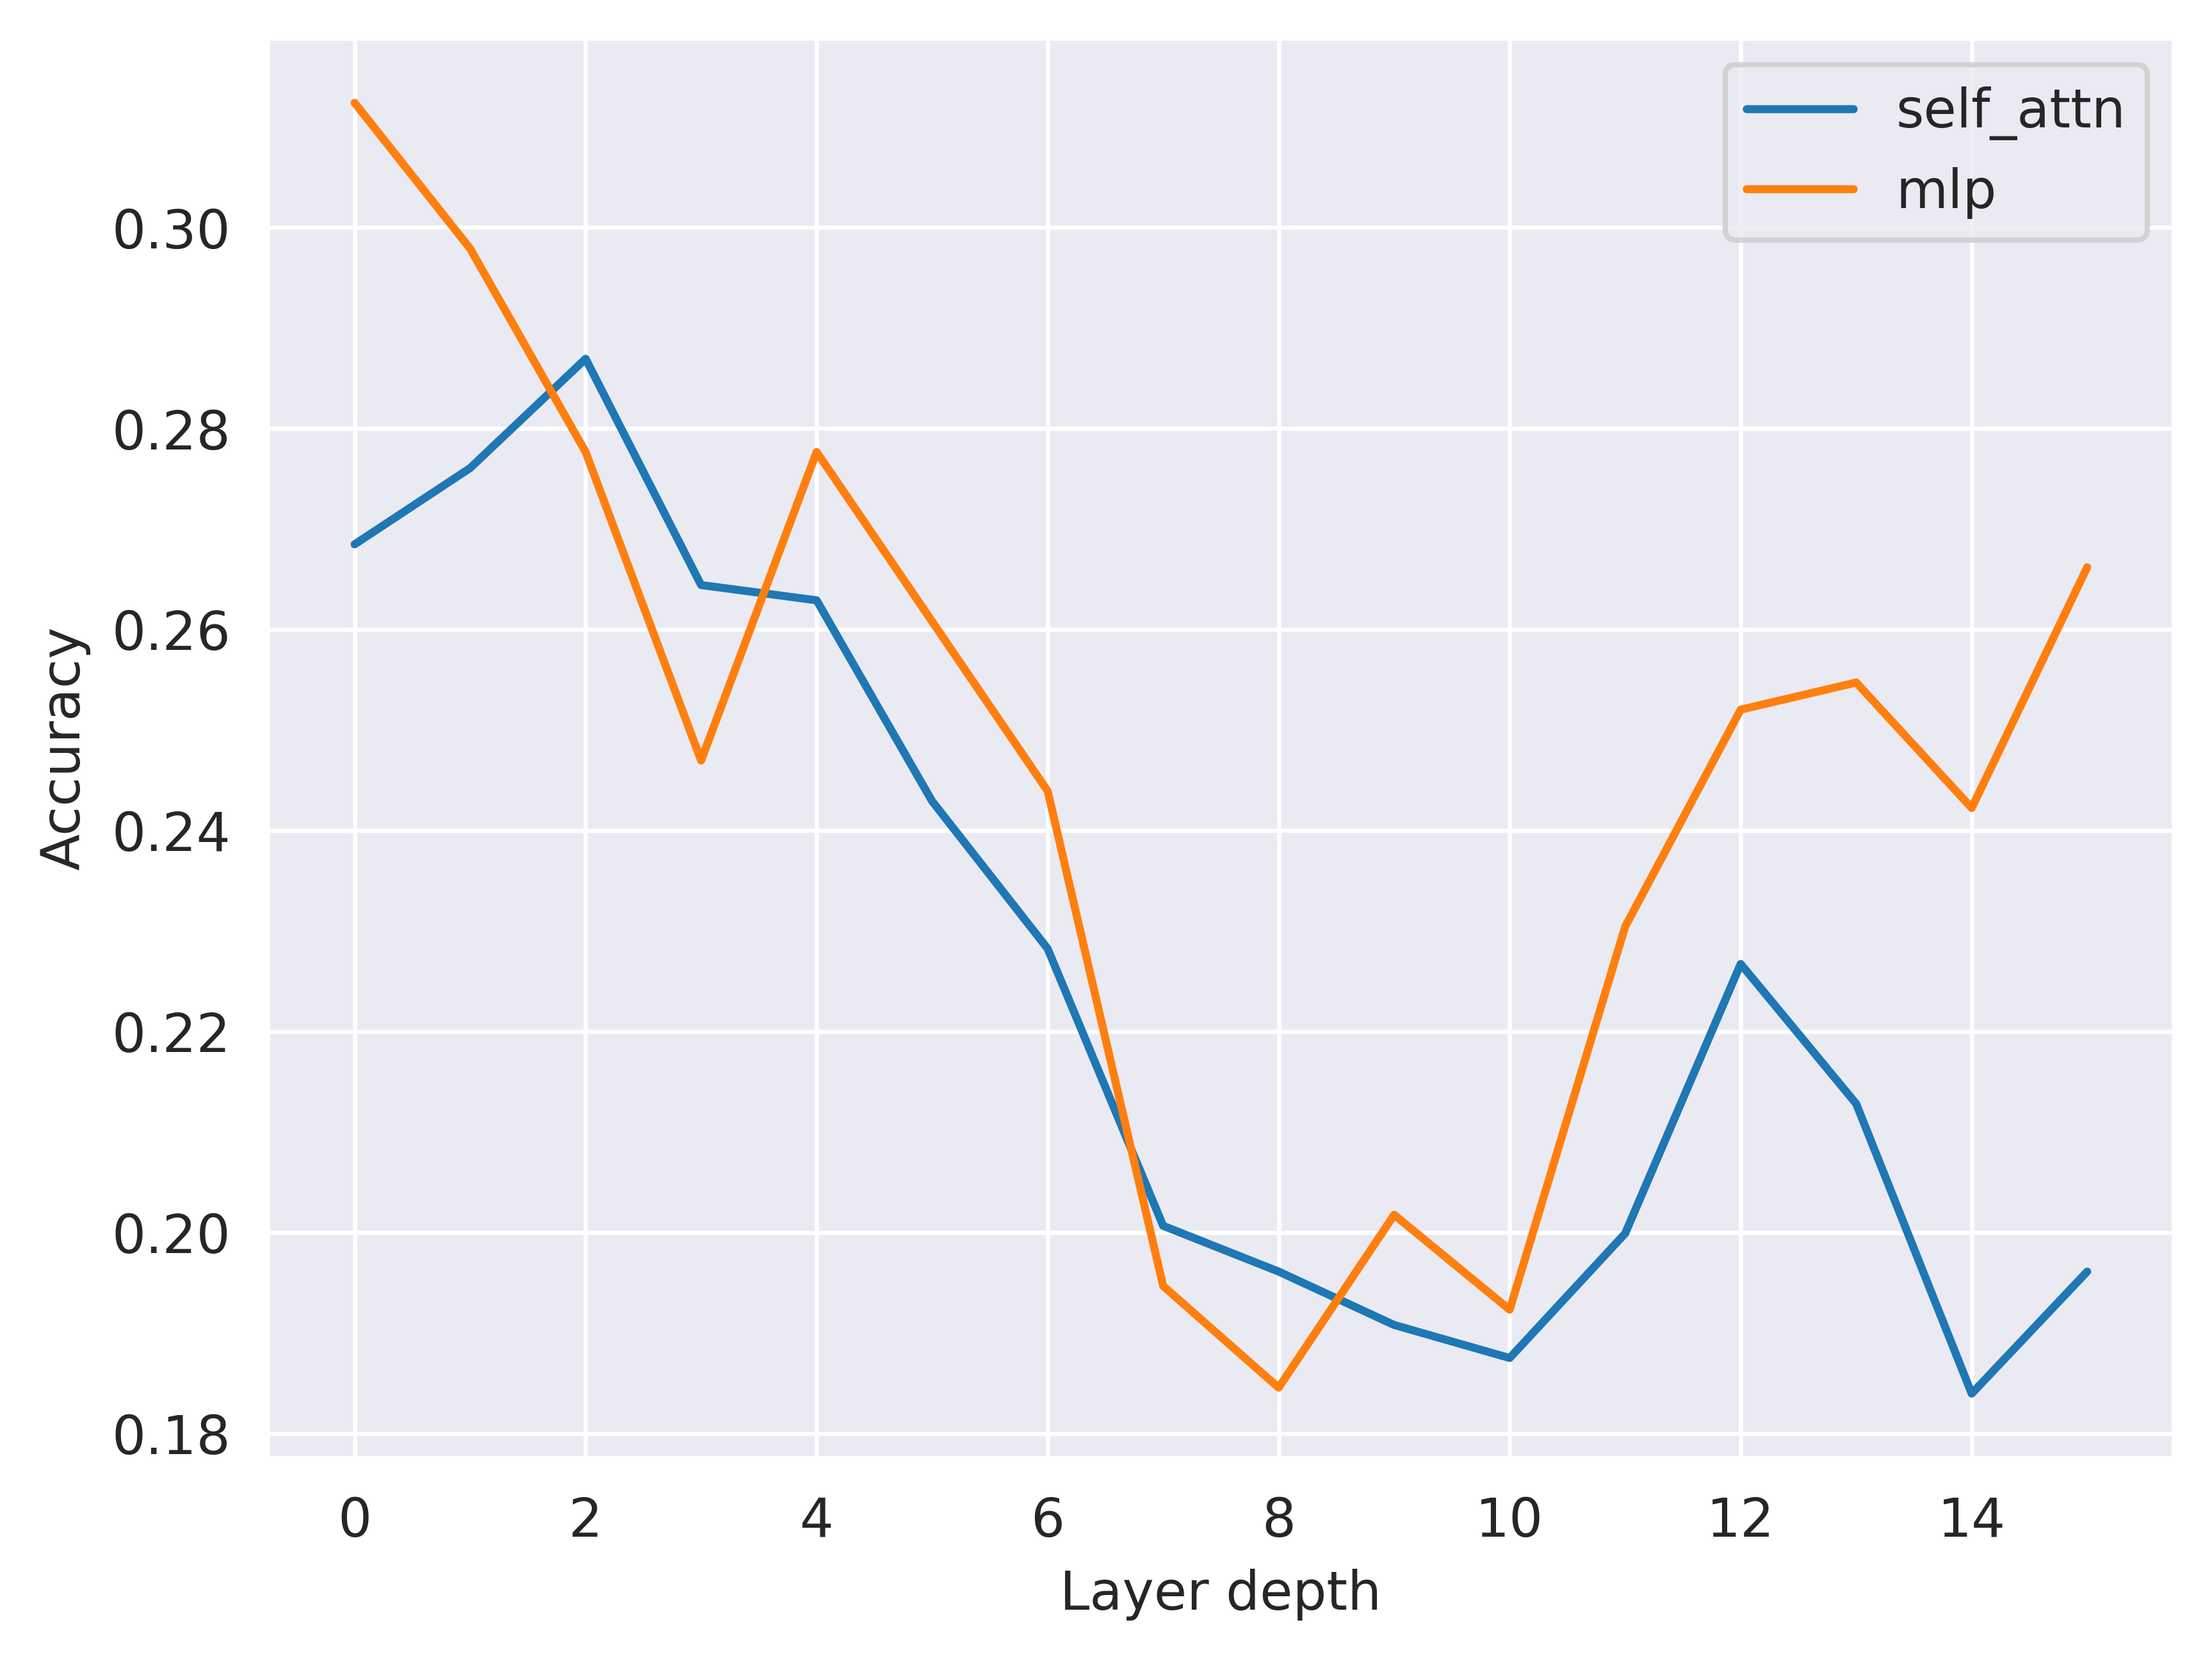
\includegraphics[width=\textwidth]{figures/results/model-generated/overall_attention_vs_mlp.png}
        \caption{Mean accuracy: Attention vs. MLP (model-generated).}             % (b)
        \label{fig:accuracy_over_layer_depth_attention_vs_mlp_model_generated}
    \end{subfigure}
    \begin{subfigure}[h]{0.49\textwidth}
        \centering
        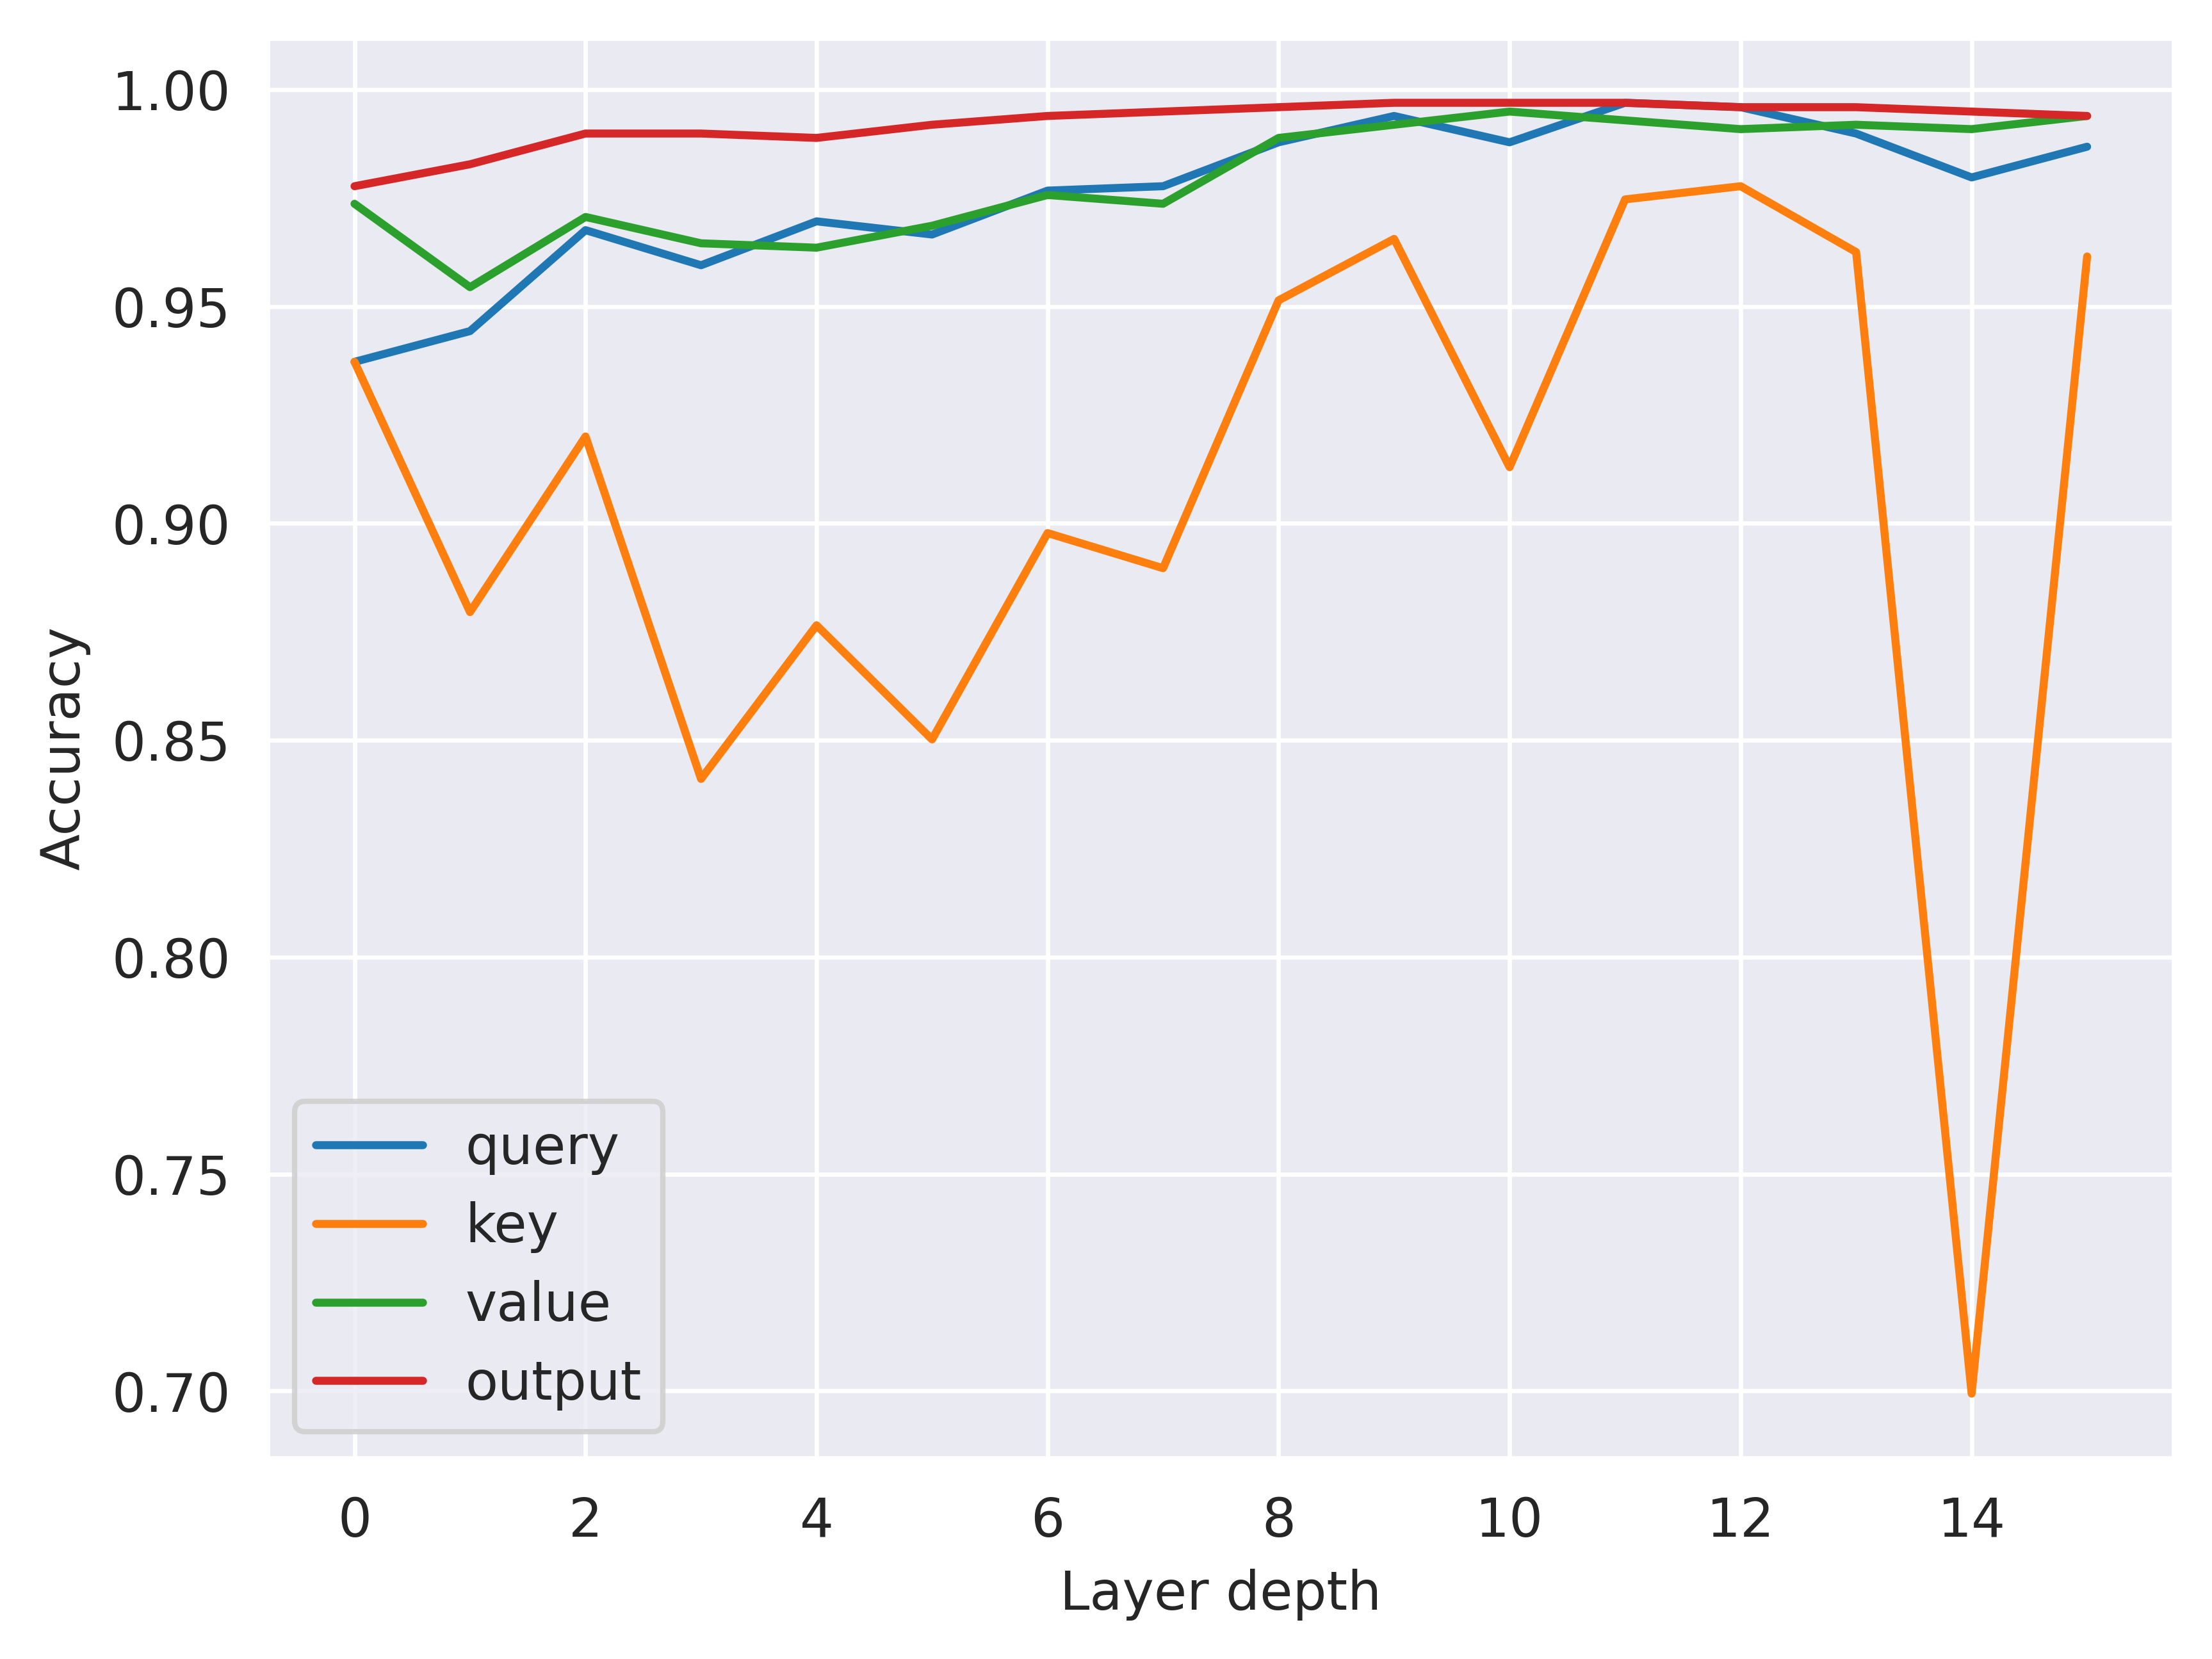
\includegraphics[width=\textwidth]{figures/results/paraphrased/attention_components.png}
        \caption{Layer-wise accuracy: Attention sub-components (Q/K/V/O), paraphrased.}      % (c)
        \label{fig:accuracy_over_layer_depth_attention_paraphrased}
    \end{subfigure}
    \hfill
    \begin{subfigure}[h]{0.49\textwidth}
        \centering
        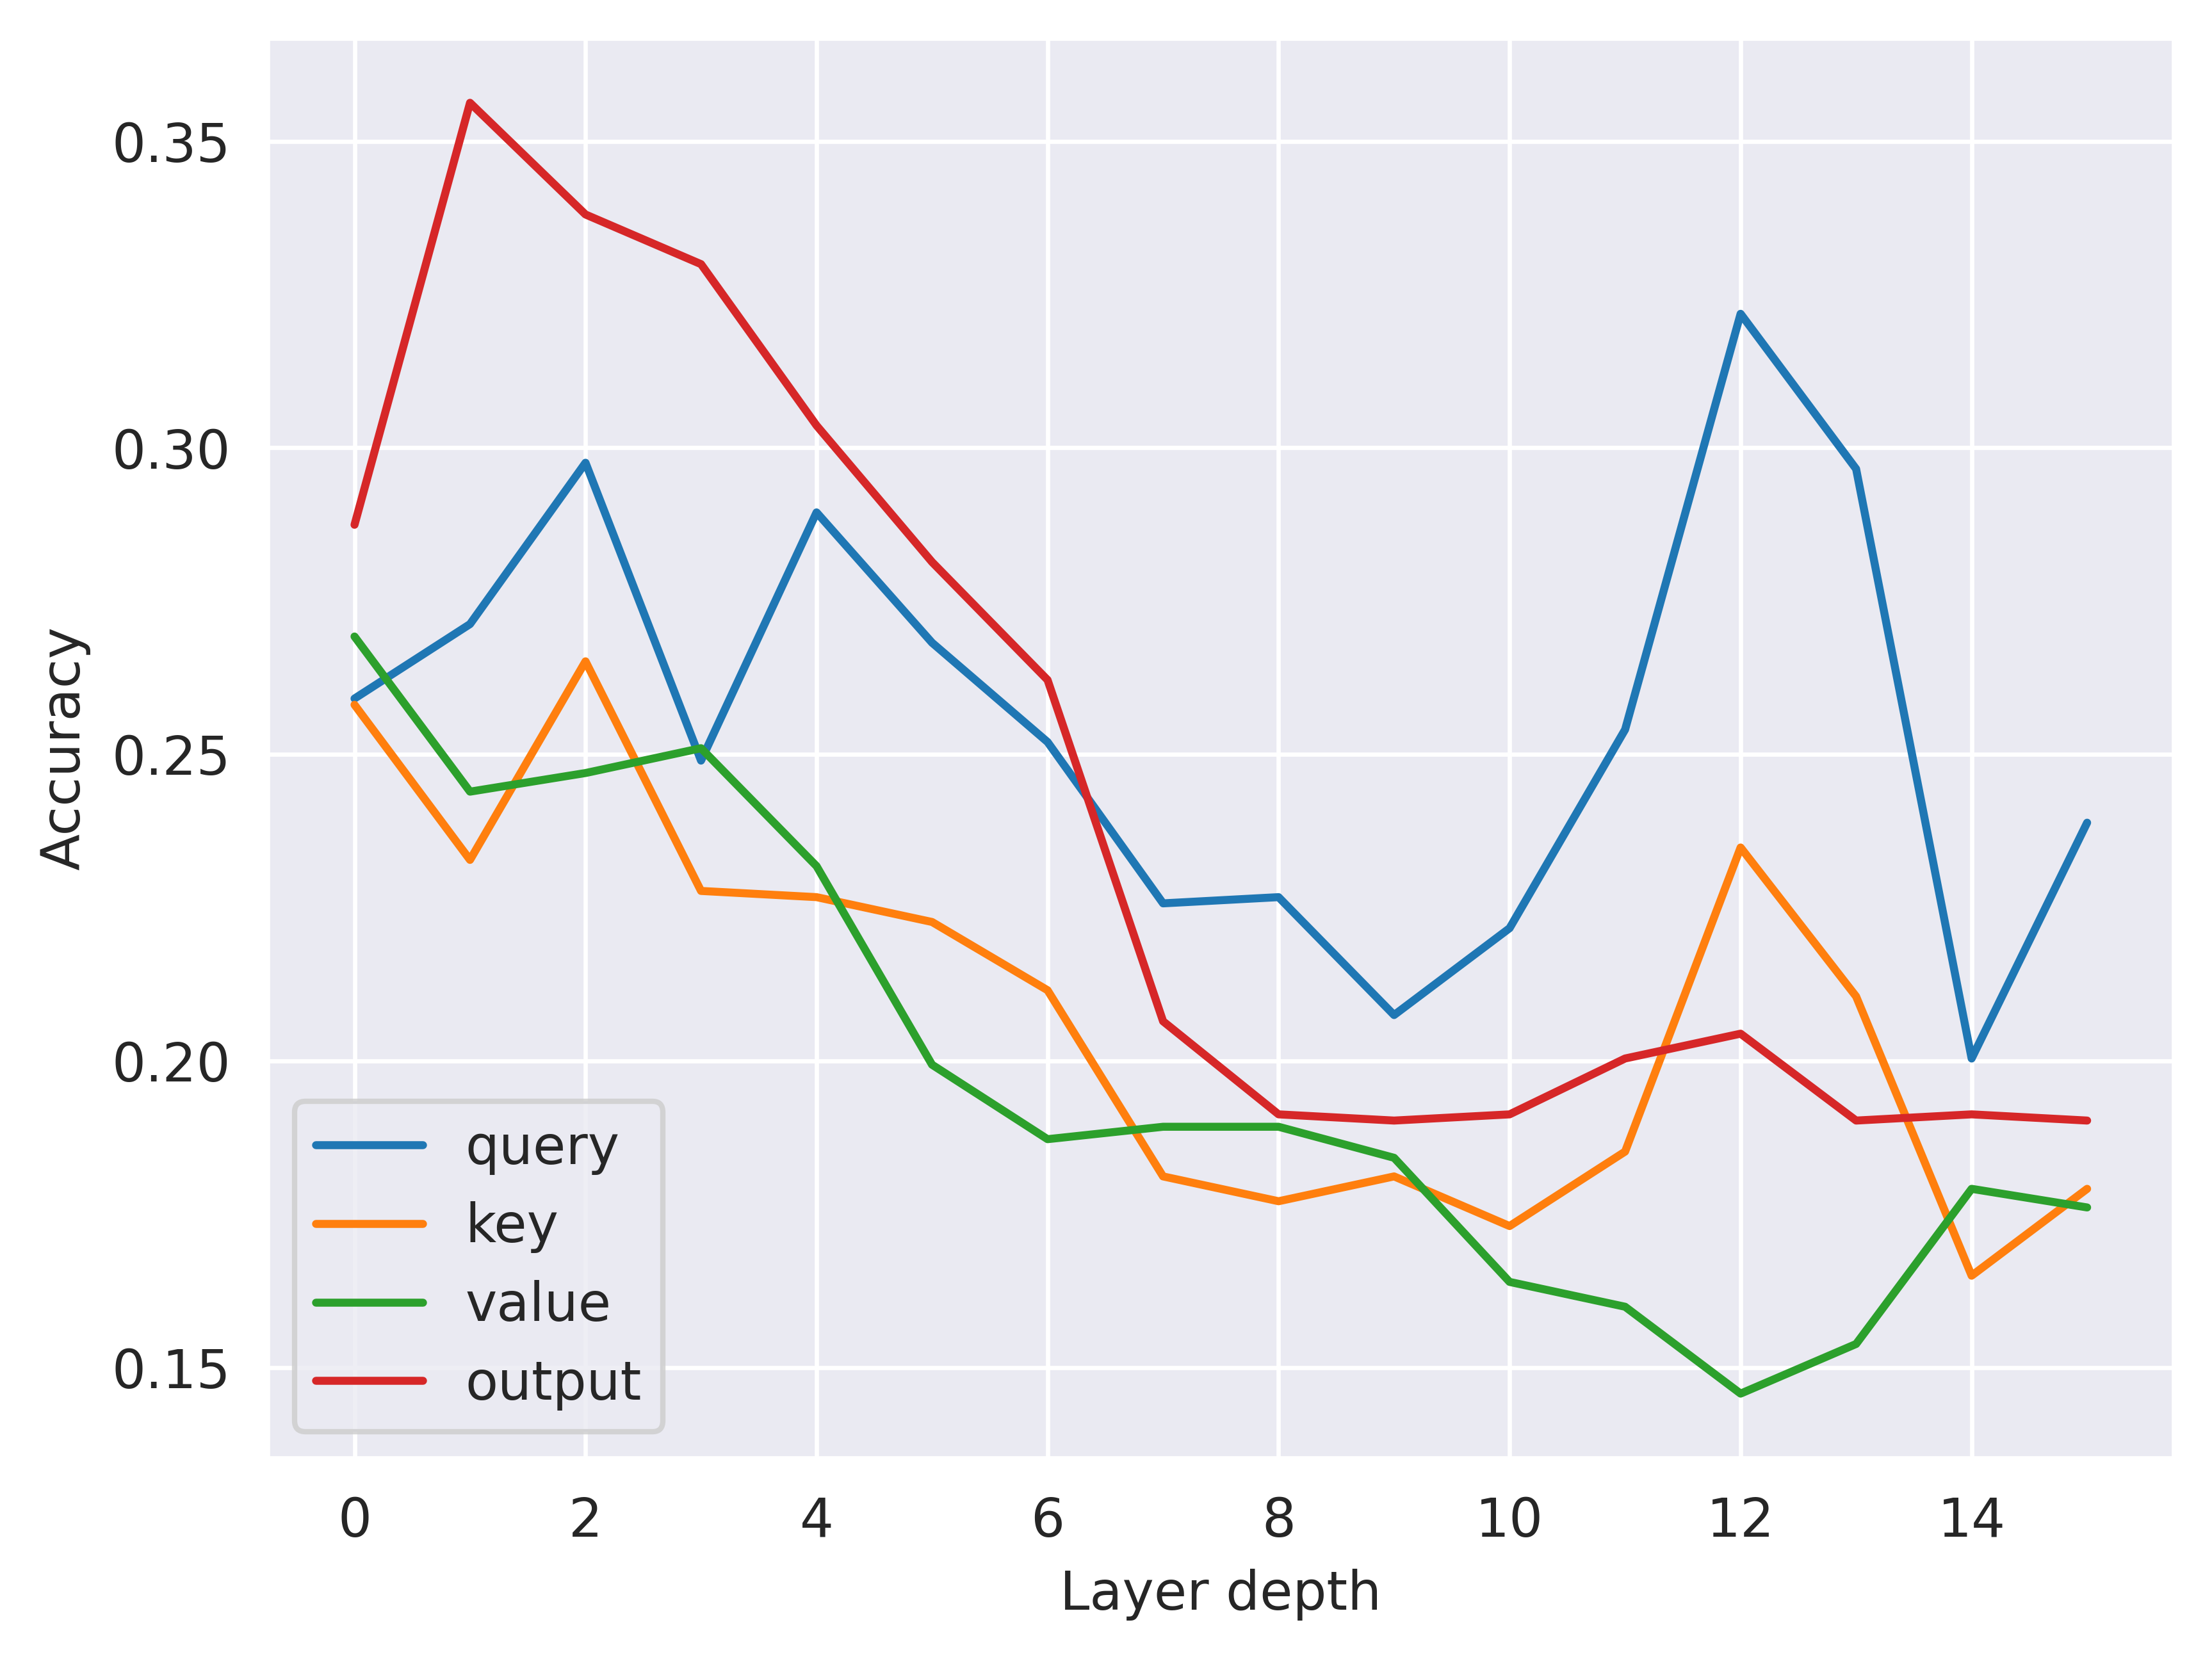
\includegraphics[width=\textwidth]{figures/results/model-generated/attention_components.png}
        \caption{Layer-wise accuracy: Attention sub-components (Q/K/V/O), model-generated.}  % (d)
        \label{fig:accuracy_over_layer_depth_model_attention_generated}
    \end{subfigure}
    \begin{subfigure}[h]{0.49\textwidth}
        \centering
        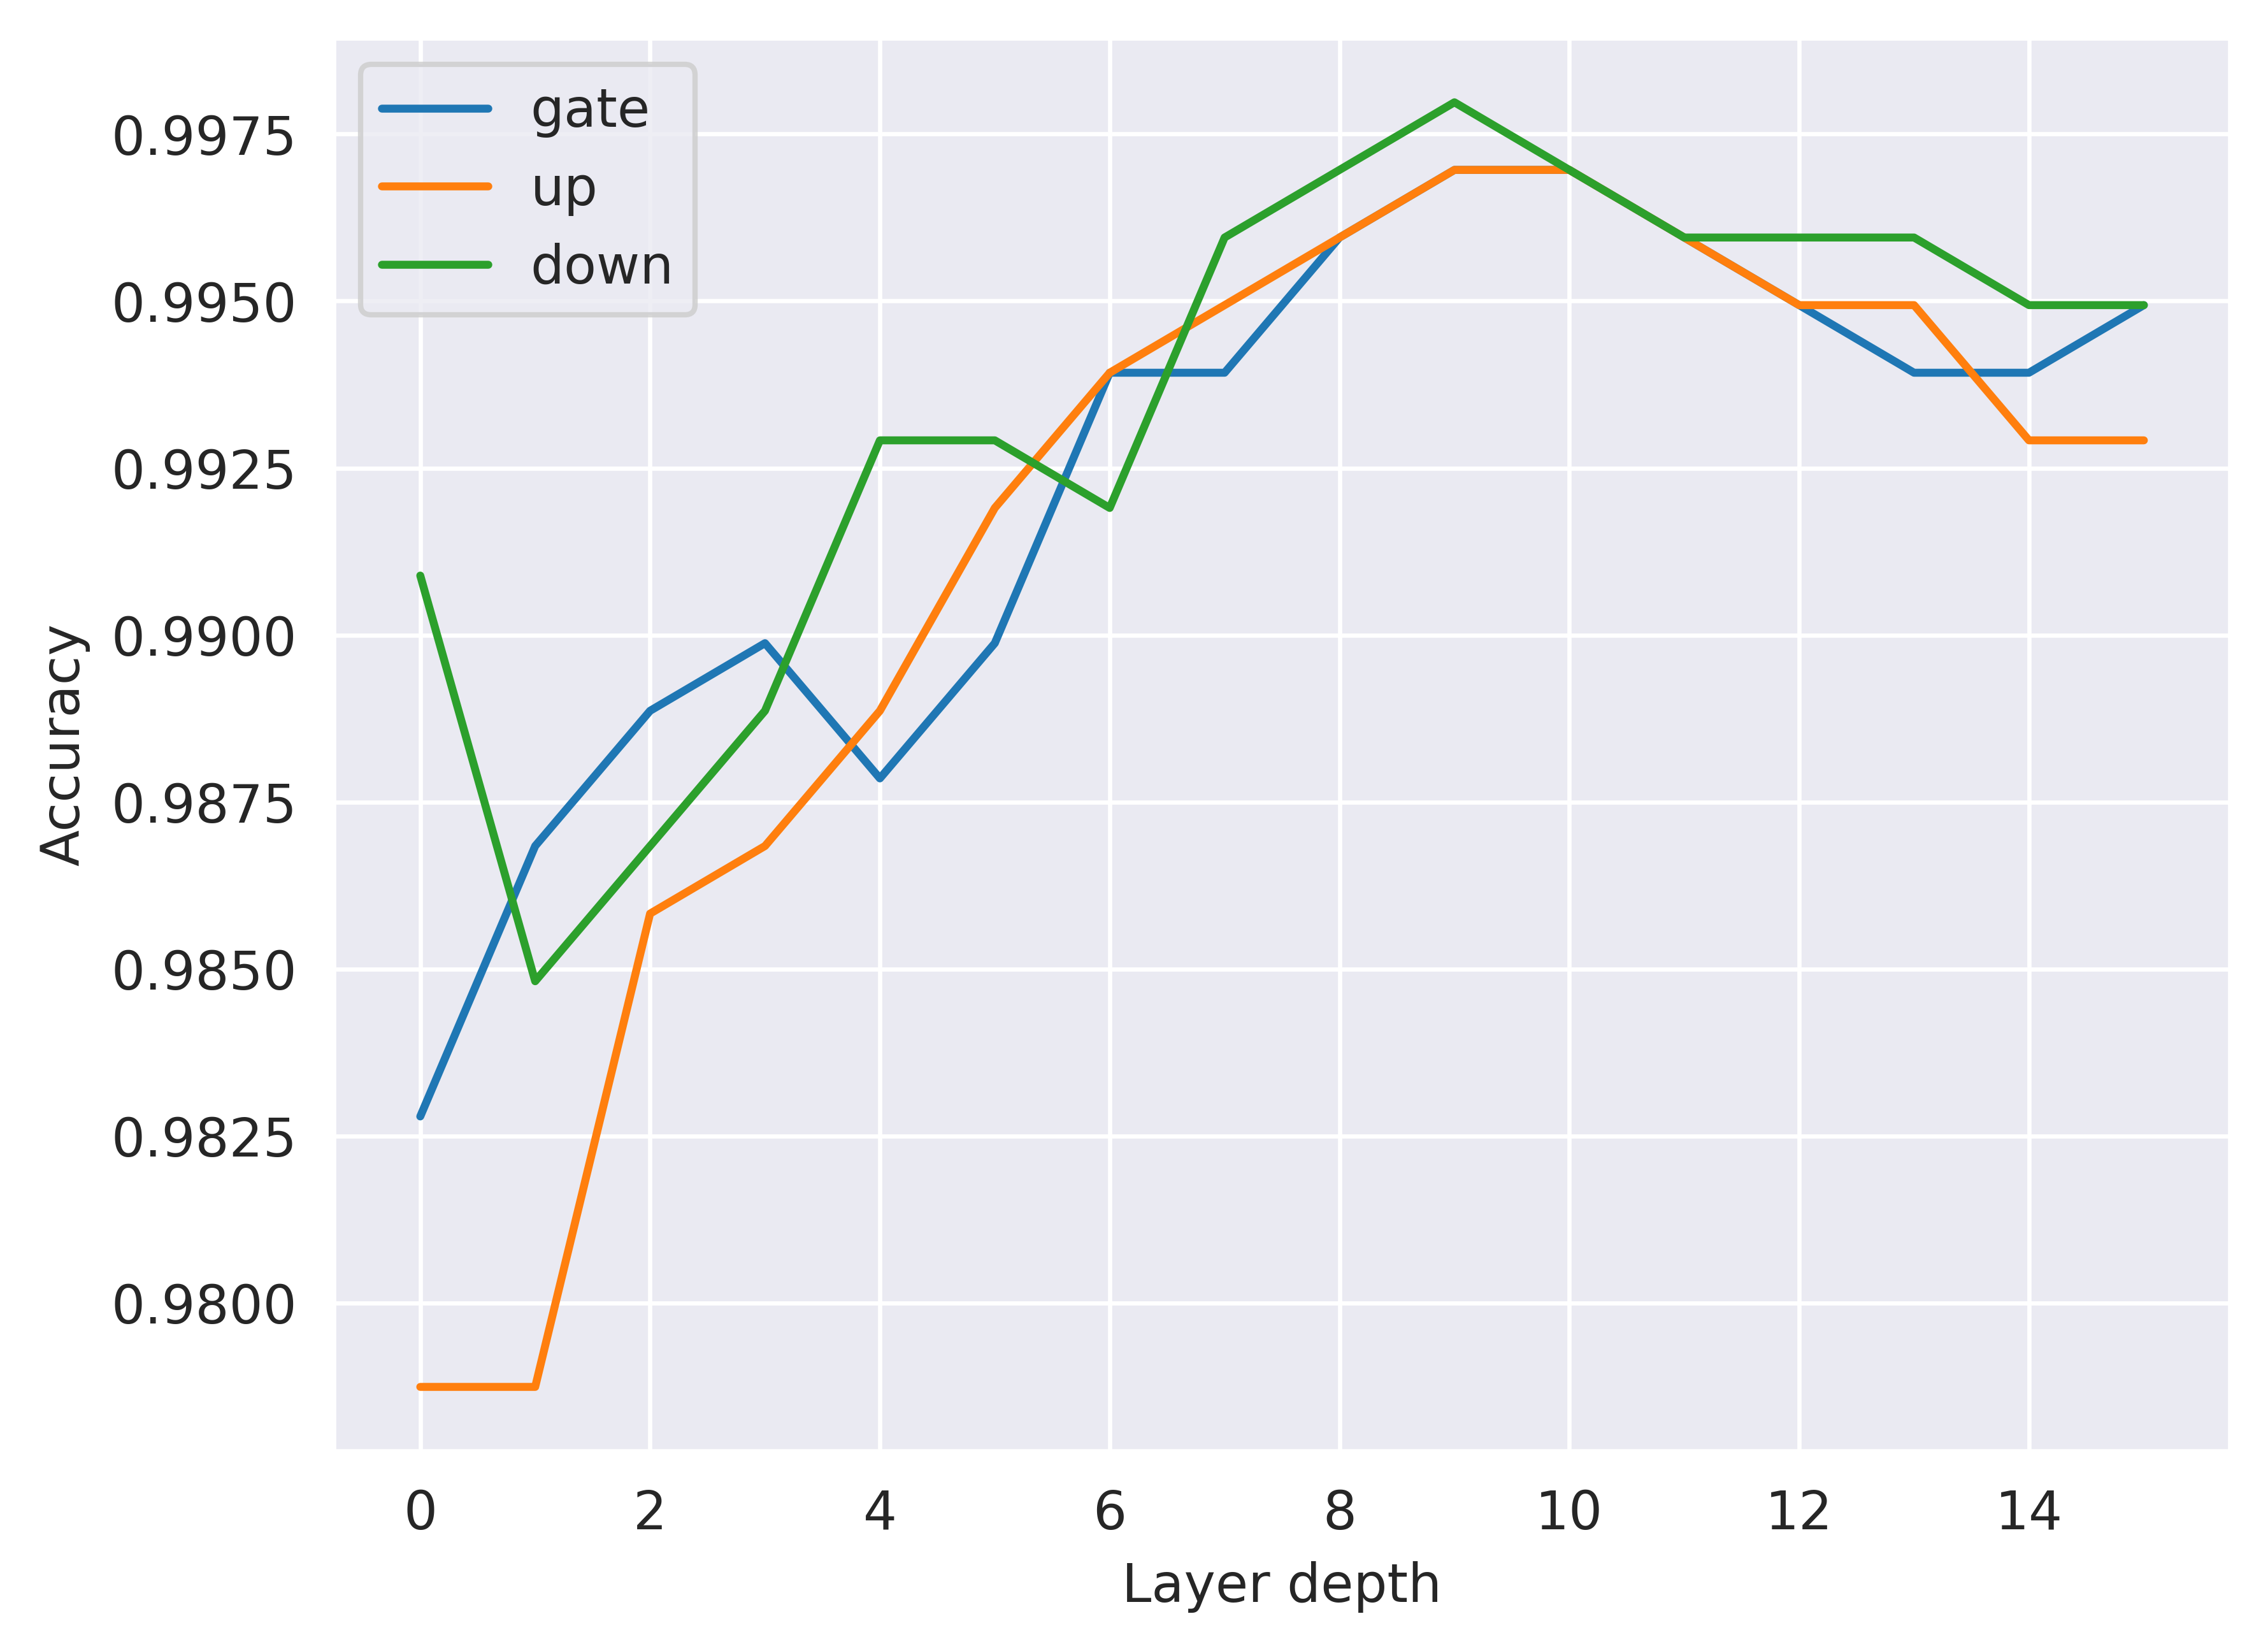
\includegraphics[width=\textwidth]{figures/results/paraphrased/mlp_components.png}
        \caption{Layer-wise accuracy: MLP sub-components (gate/up/down), paraphrased.}       % (e)
        \label{fig:accuracy_over_layer_depth_mlp_paraphrased}
    \end{subfigure}
    \hfill
    \begin{subfigure}[h]{0.49\textwidth}
        \centering
        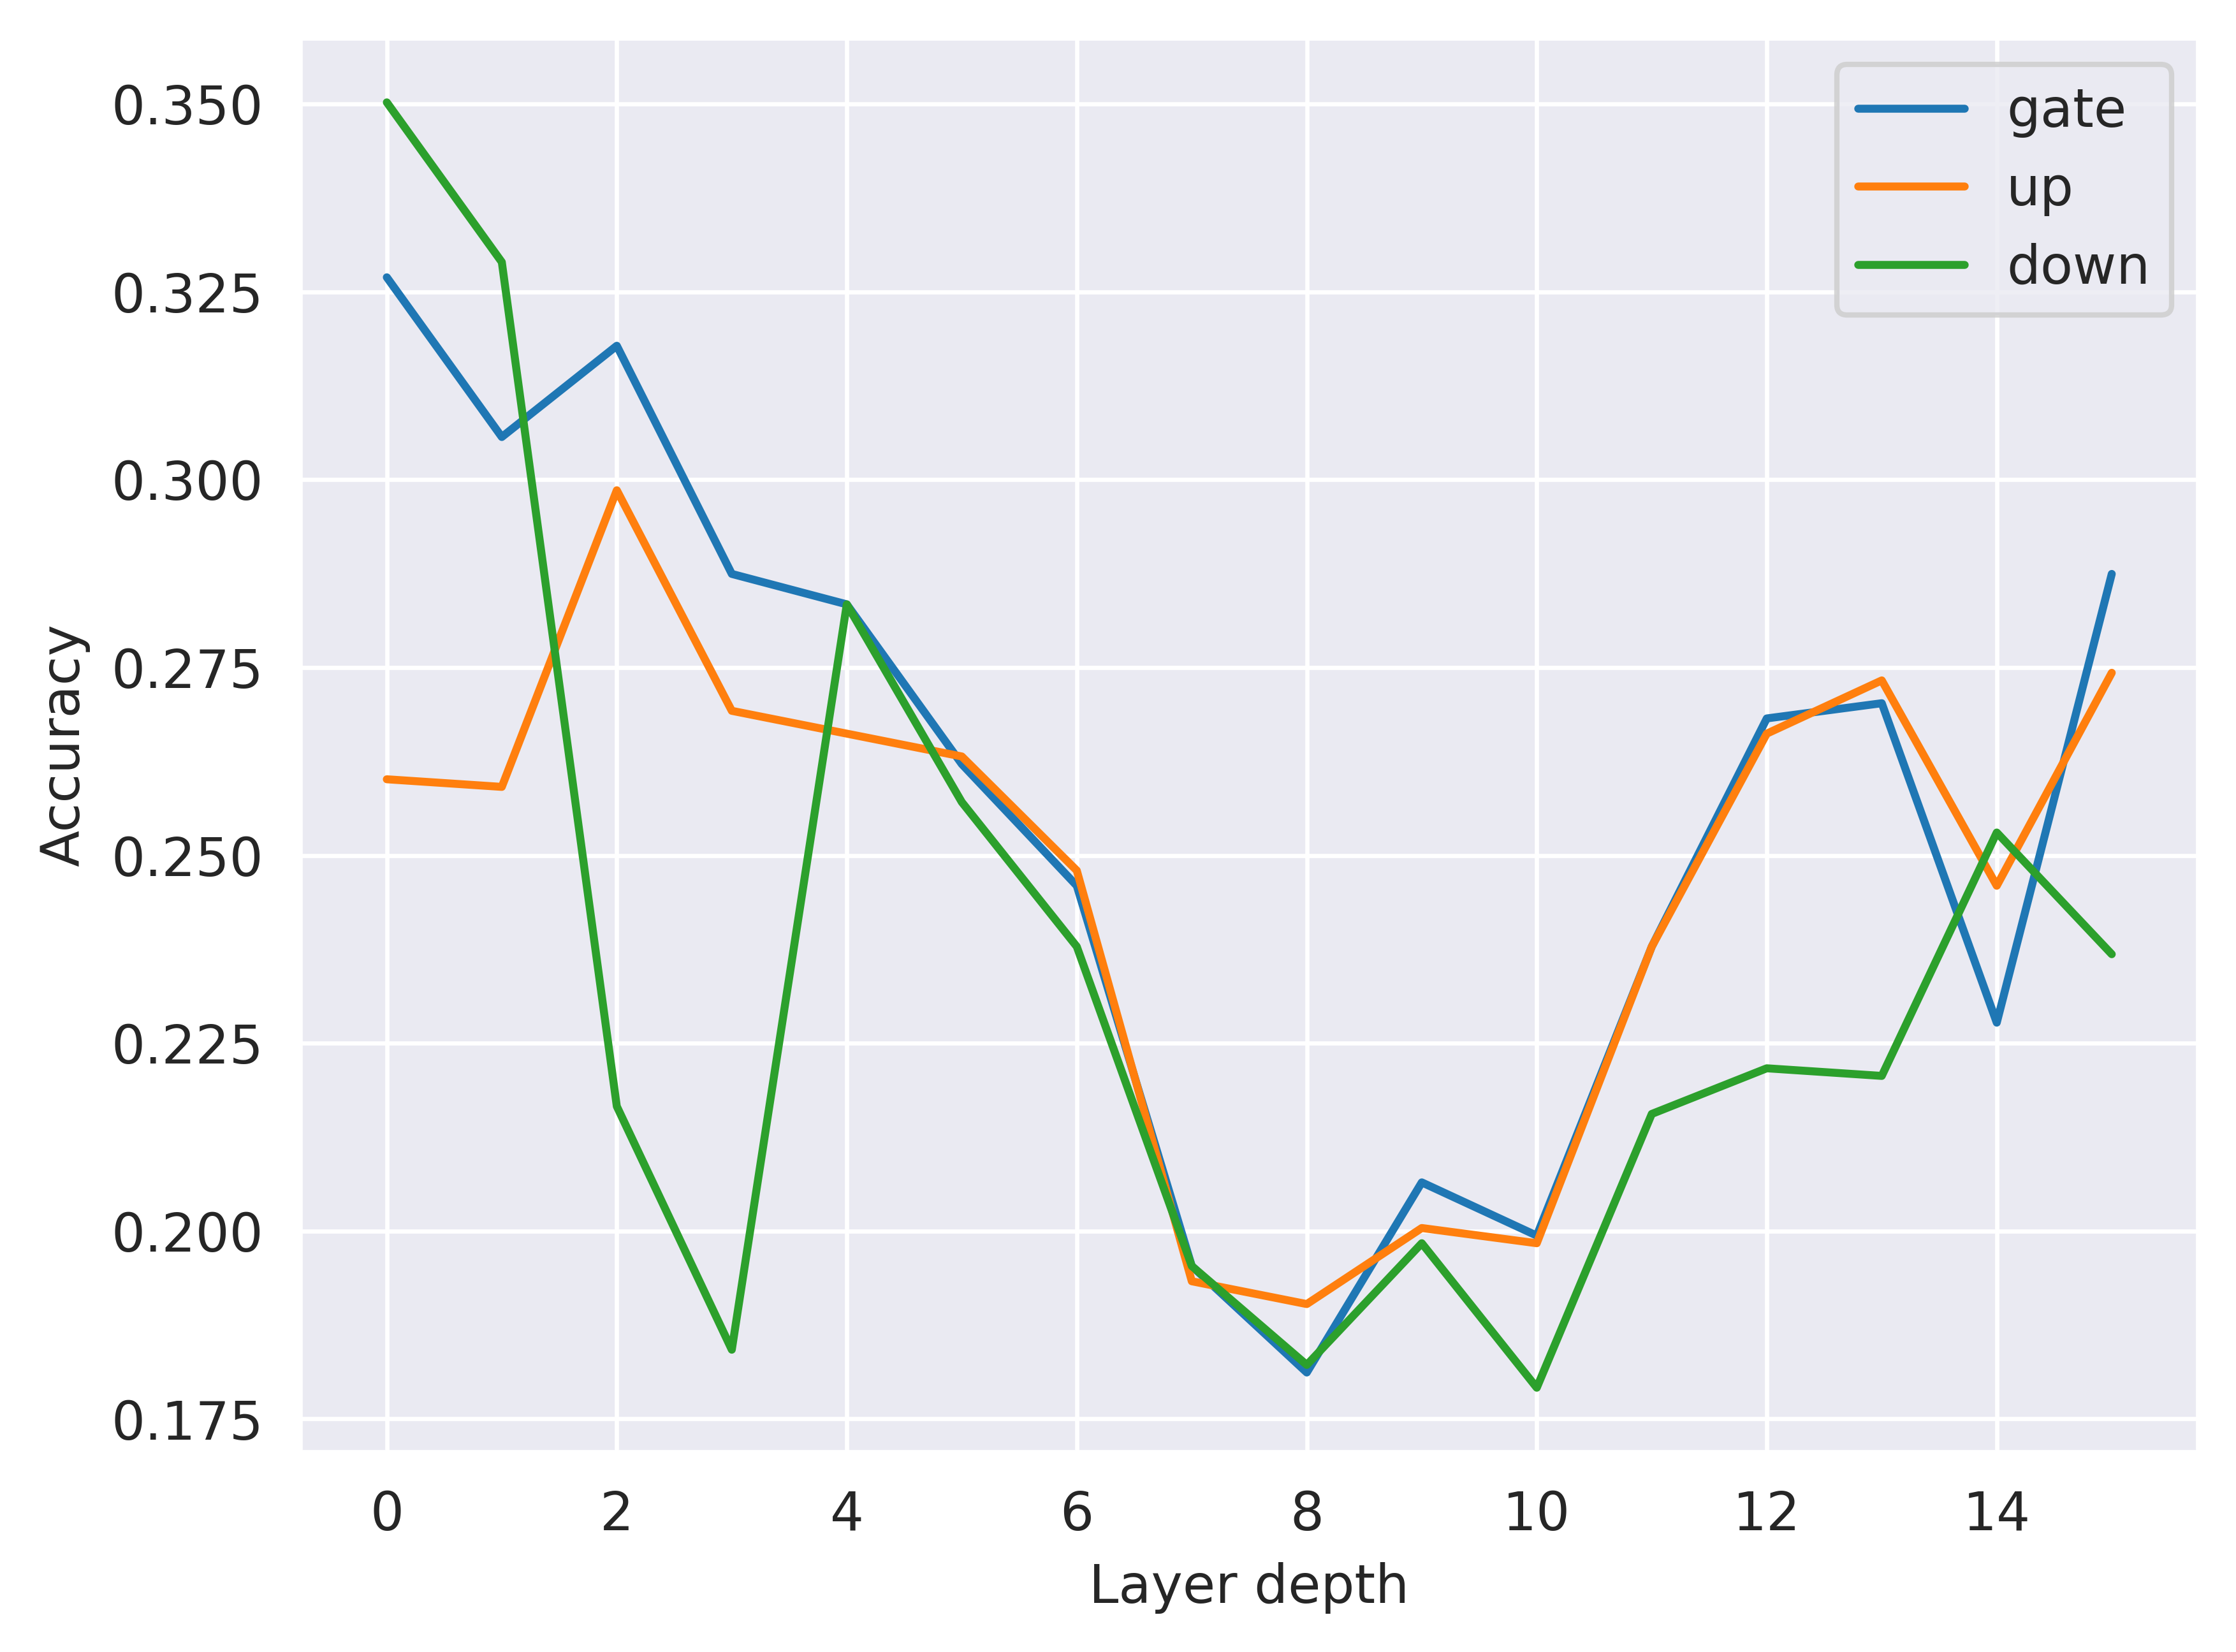
\includegraphics[width=\textwidth]{figures/results/model-generated/mlp_components.png}
        \caption{Layer-wise accuracy: MLP sub-components (gate/up/down), model-generated.}   % (f)
        \label{fig:accuracy_over_layer_depth_mlp_model_generated}
    \end{subfigure}
    \caption{Accuracy over layer depth ($l = 0, \ldots, 15$). Left: paraphrased; right: model-generated. Panels (a,b): mean over sub-components; panels (c–f): per-sub-component layer-wise accuracy.}
    \label{fig:accuracy_over_layer_depth}
\end{figure}

\section{Comparison of Layer-Gradients and Full-Model-Gradient}\label{sec:layer_vs_full}
With the full-model and single-layer accuracies established for the paraphrased and model-generated settings, the subsequent analysis compares each single-layer component against the full-model gradient. This is done by looking at the cosine-similarity between the different scores values $\simcos(\hat{\Gamma}^{\mathcal{L}},\Gamma^\theta)$ (Equation~\ref{eq:rho_objective}).
\begin{table}[H]
    \centering
    \begin{tabular}{|c|c|c|c|}
        \hline
        & \textbf{Layer Component} & \textbf{Paraphrased} & \textbf{Model-generated} \\
        \hline
        \multirow{1}{5em}{Embedding}
        & Embedding & 0.981 & 0.275 \\
        \hline
        \multirow{4}{5em}{Attention}
        & Query-Projection & 0.972 & 0.275 \\
        & Key-Projection & 0.9 & 0.201 \\
        & Value-Projection & 0.978 & 0.62 \\
        & Output-Projection & 0.988 & 0.63 \\
        \hline
        \multirow{3}{5em}{MLP}
        & Gate-Projection & 0.986 & 0.553 \\
        & Up-Projection & 0.988 & 0.571 \\
        & Down-Projection & 0.989 & 0.63 \\
        \hline
    \end{tabular}
    \caption{Average (median) cosine similarity between the scores of single layer components ($\hat{\Gamma}^{\mathcal{L}}$) and the full gradient ($\Gamma^\theta$).}
    \label{tab:average_cosine_similarity_full_gradient_comparison}
\end{table}
\noindent Based on Table~\ref{tab:average_cosine_similarity_full_gradient_comparison}, the single components most similar to the full-model gradient in the \emph{paraphrased} setting are the MLP projections and the attention output projection: {MLP down} $0.989$, {MLP up} $0.988$, {Attention output} $0.988$, {MLP gate} $0.986$; the embedding ($0.981$) and Attention value ($0.978$) follow, with Attention query at $0.972$ and Attention key lowest at $0.900$. In the \emph{model-generated} setting, the highest agreements are {Attention output} and {MLP down} (both $0.630$), then Attention value ($0.620$) and MLP up ($0.571$), with MLP gate at $0.553$; embedding and Attention query are much lower (both $0.275$), and Attention key is weakest ($0.201$).

\section{Greedy-Forward-Layer-Selection vs. Random Projections}\label{sec:greedy_vs_rp}
Two forward greedy strategies are evaluated using the precomputed dot products: (i) a \emph{similarity-driven} variant (Alg.~\ref{alg:greedy_layer_selection}) that maximizes agreement with the full-model score vector $\Gamma^\theta$ (objective $\rho$ in Eq.~\ref{eq:rho_objective}), and (ii) an \emph{accuracy-driven} variant (Alg.~\ref{alg:greedy_layer_selection_accuracy}) that directly maximizes BM25-restricted top-1 retrieval accuracy (Eq.~\ref{eq:accuracy_bm25_reconstructed}). As a geometry-preserving baseline, layer-wise random projections (Sec.~\ref{subsec:random_projection_as_a_baseline}) are applied at 1\% and 5\% of $M$. Budgets on the $x$-axis are reported as the cumulative fraction of selected model parameters.

\subsection{Selection by Accuracy}
Figure~\ref{fig:greedy_layer_selection_accuracy} shows $\operatorname{accuracy}^{(b)}$ as layers are added.
In the \emph{paraphrased} case (Fig.~\ref{fig:greedy_layer_selection_accuracy_paraphrased}), greedy selection reaches near-ceiling accuracy with a very small budget ($\approx0.998$ at $\ll10\%$ of parameters) and then slightly declines as additional components are appended, ending close to the full-model score ($\approx0.993$). The random-projection baselines at 1\% and 5\% lie around $0.994$, below the early greedy frontier. In the \emph{model-generated} case (Fig.~\ref{fig:greedy_layer_selection_accuracy_model_generated}), accuracy peaks around $0.35$–$0.36$ for small budgets and gradually drifts toward $\approx0.22$ as more parameters are added; the 1\%/5\% random-projection baselines are near the $0.2$ candidate-set chance level and are dominated by the greedy curve for small–to–medium budgets. Overall, adding more components does not necessarily improve retrieval—weakly aligned layers can dilute the signal captured by the strongest ones.
\begin{figure}[H]
    \centering
    \begin{subfigure}[h]{0.49\textwidth}
        \centering
        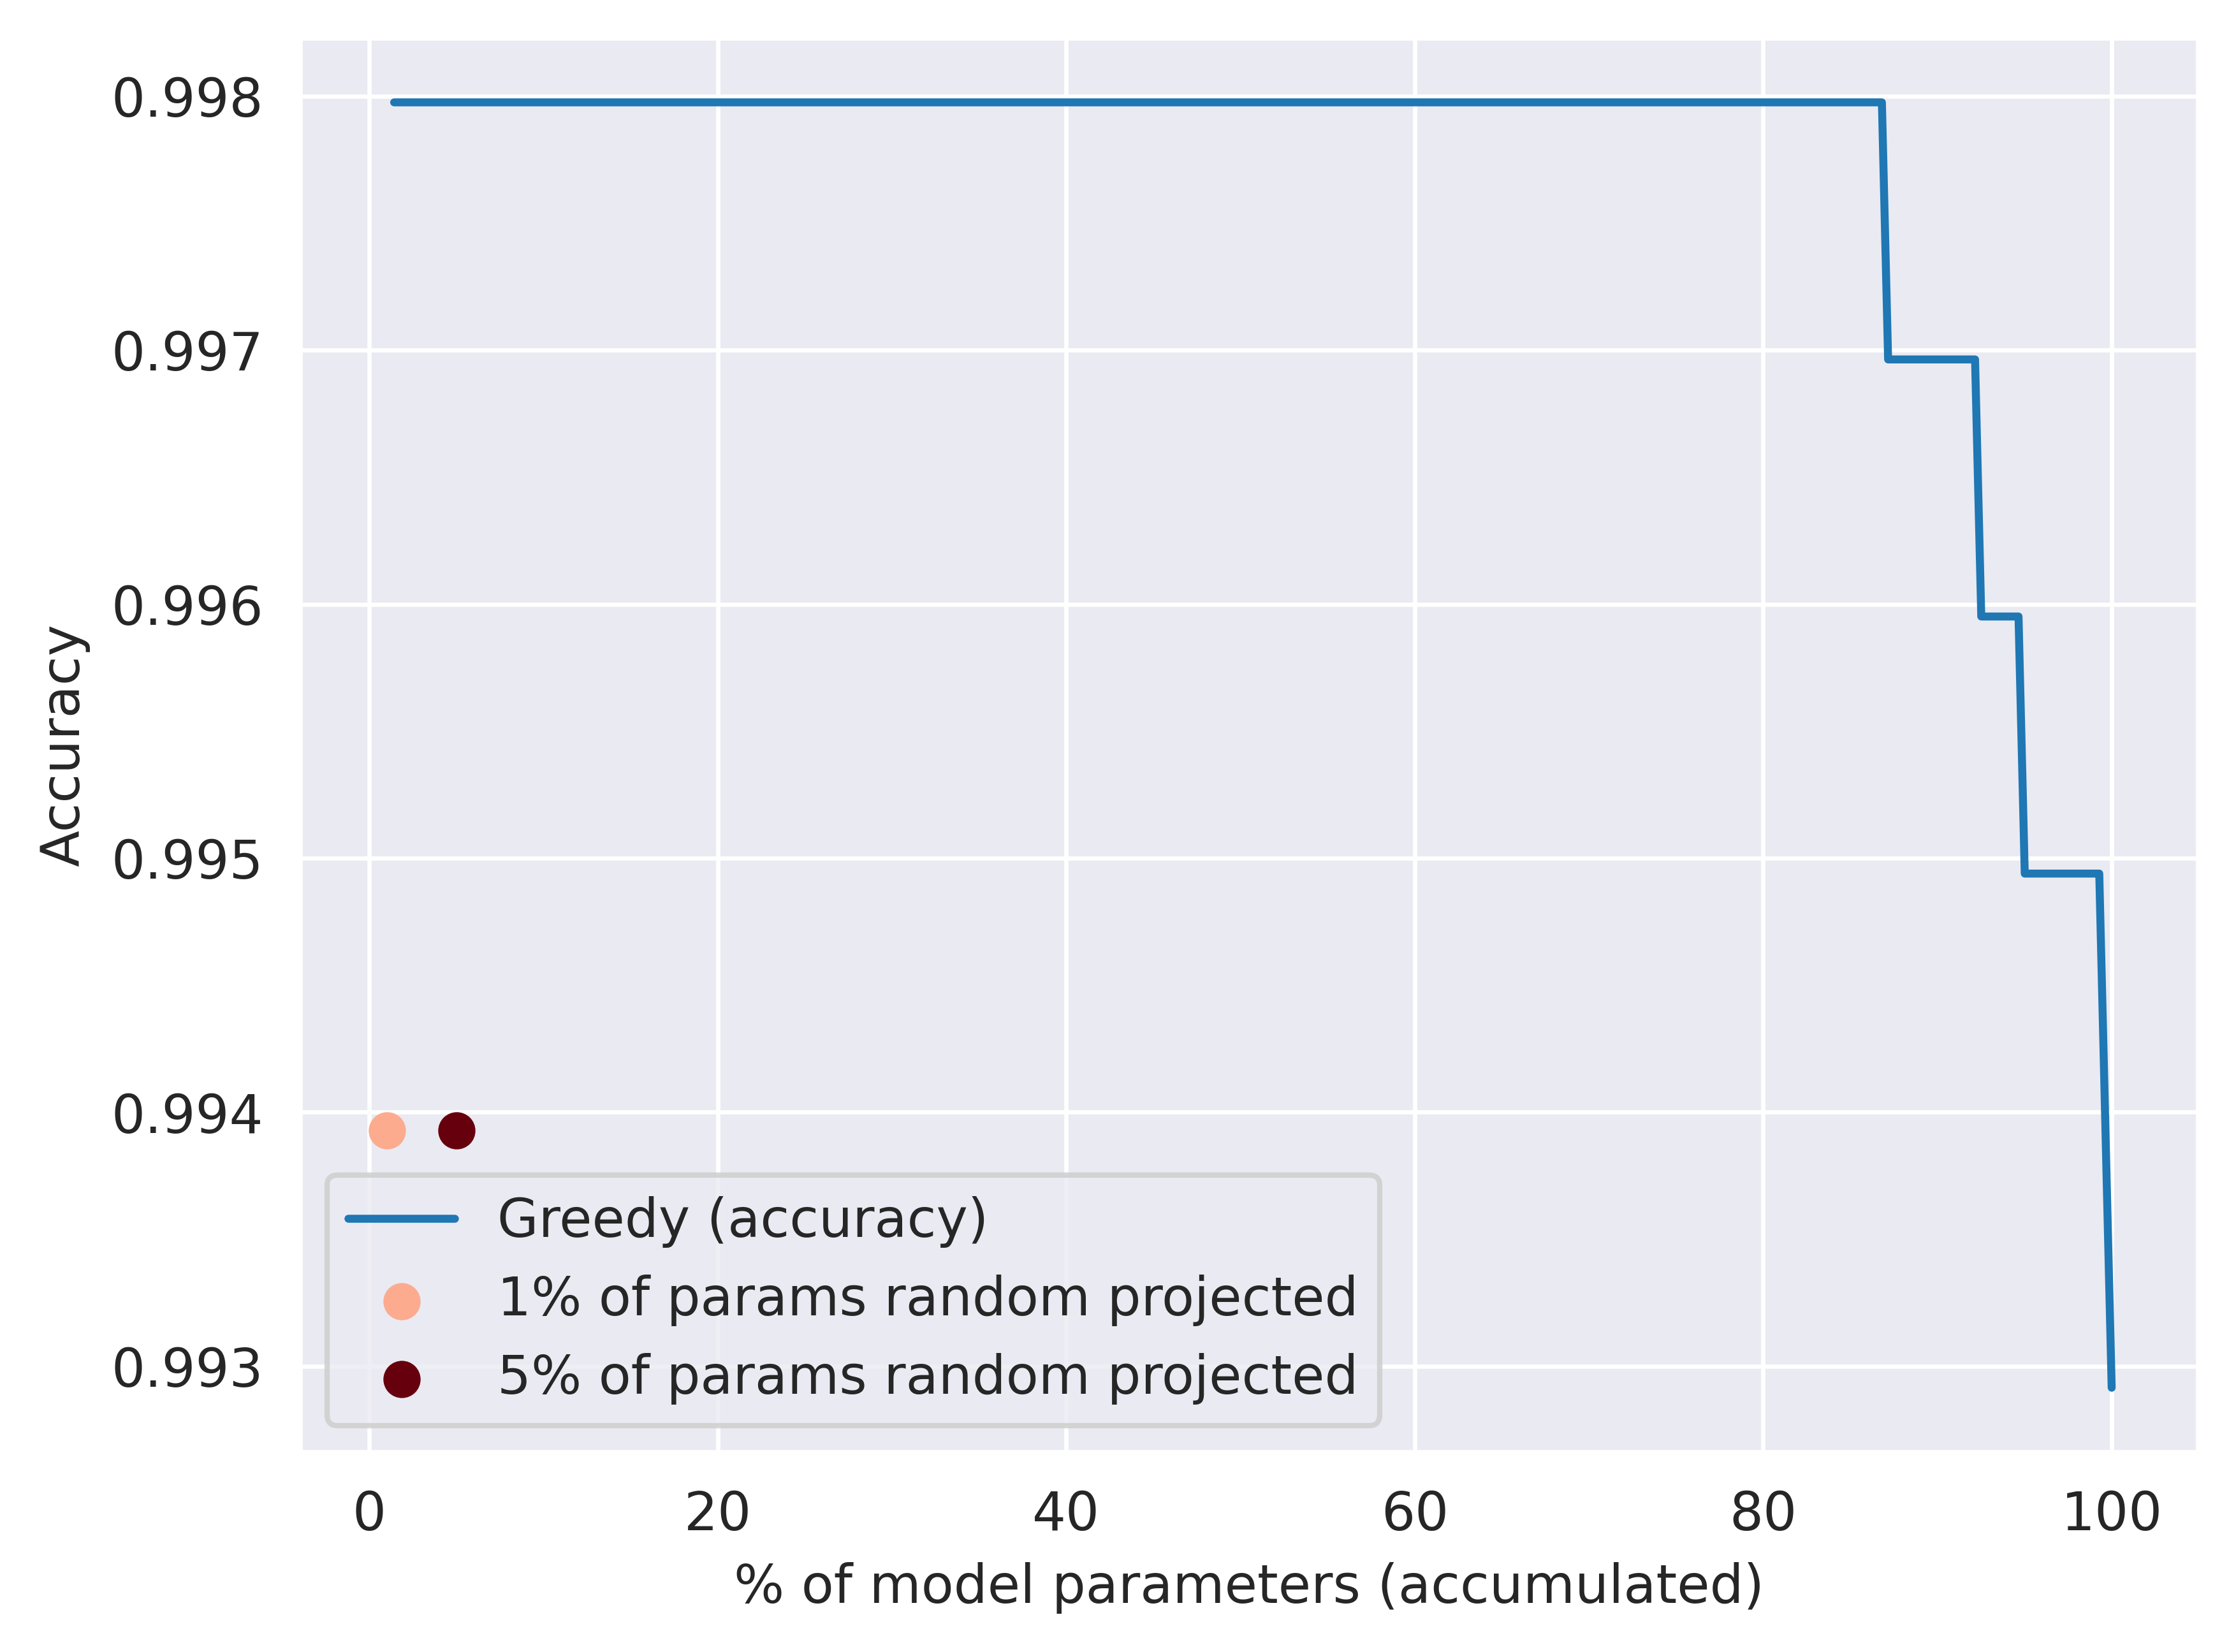
\includegraphics[width=\textwidth]{figures/results/paraphrased/greedy_layer_selection_accuracy.png}
        \caption{Paraphrased}
        \label{fig:greedy_layer_selection_accuracy_paraphrased}
    \end{subfigure}
    \hfill
    \begin{subfigure}[h]{0.49\textwidth}
        \centering
        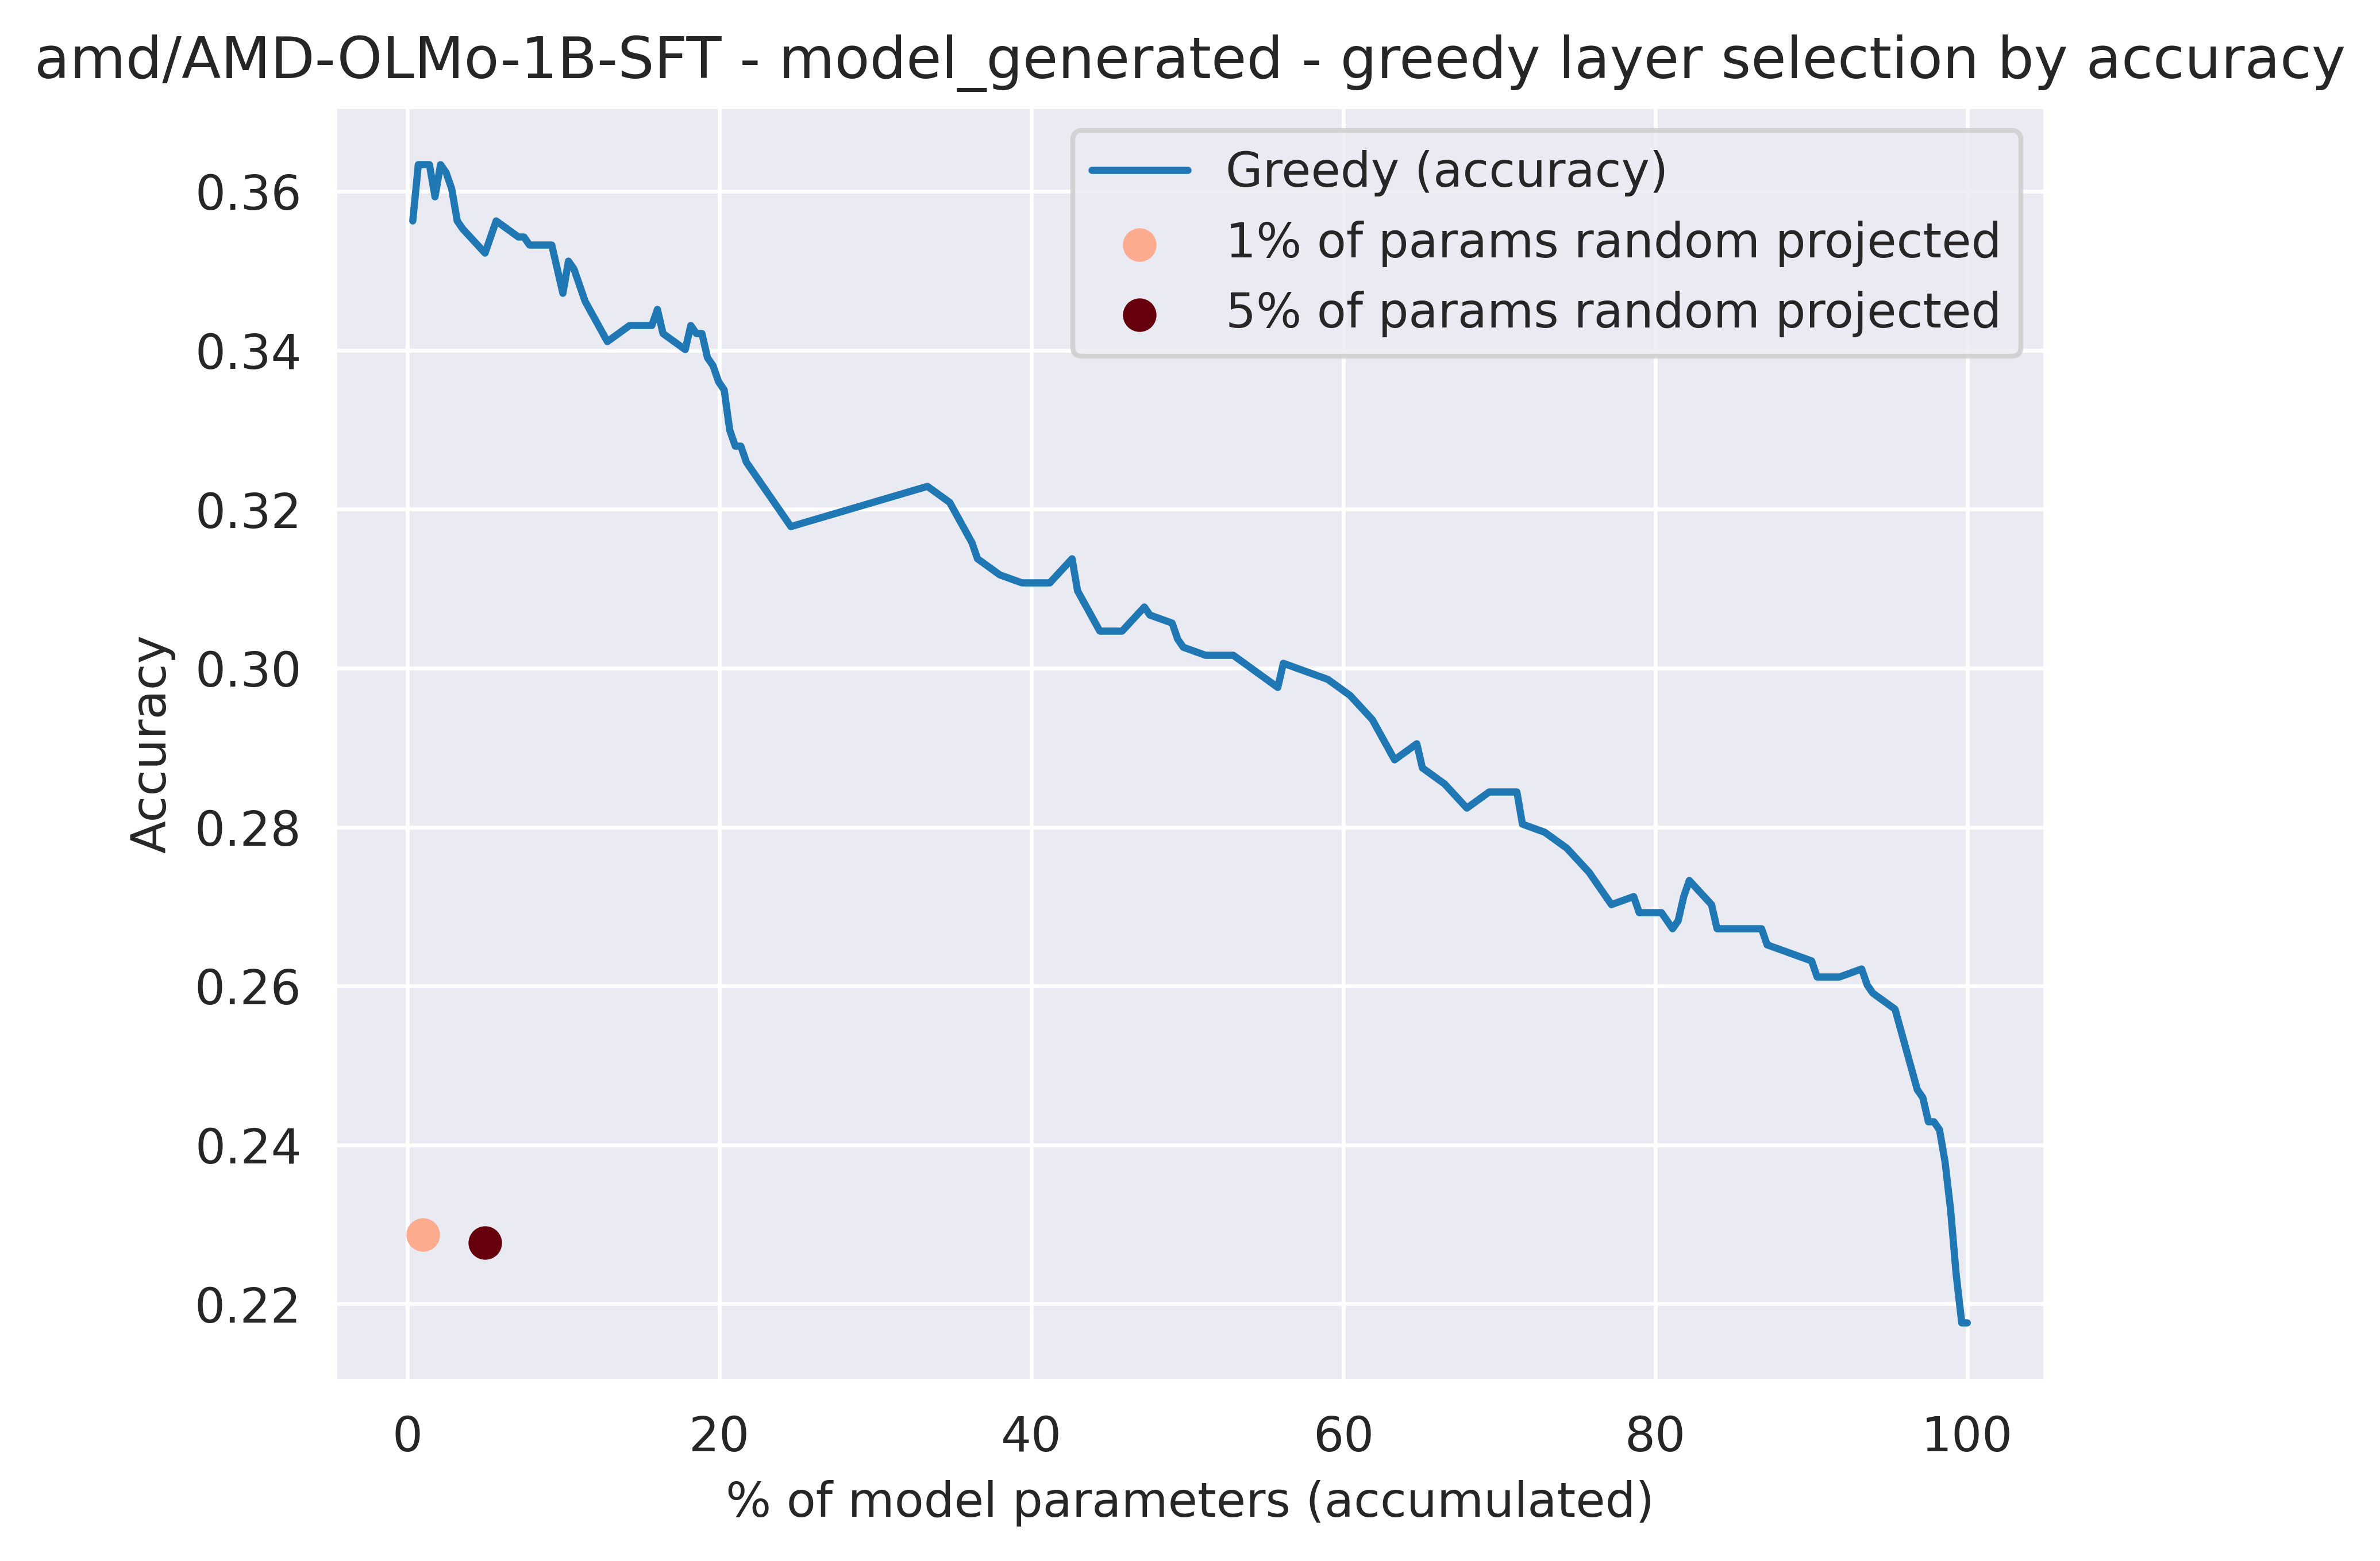
\includegraphics[width=\textwidth]{figures/results/model-generated/greedy_layer_selection_accuracy.png}
        \caption{Model-generated}
        \label{fig:greedy_layer_selection_accuracy_model_generated}
    \end{subfigure}
    \caption{Greedy Layer Selection and random projection by accuracy.}
    \label{fig:greedy_layer_selection_accuracy}
\end{figure}

\subsection{Selection by Similarity to the Full-Model Gradient}
Figure~\ref{fig:greedy_layer_selection} tracks $\rho(\mathcal{L})=\simcos(\hat{\Gamma}^{\mathcal{L}},\Gamma^\theta)$ while components are added.
For \emph{paraphrased} data (Fig.~\ref{fig:greedy_layer_selection_paraphrased}), similarity jumps to $>0.999$ within a tiny budget and monotonically approaches $1.0$ as layers accumulate; 1\% and 5\% random projections land around $0.999$ but remain below the greedy trajectory. For \emph{model-generated} data (Fig.~\ref{fig:greedy_layer_selection_model_generated}), similarity climbs rapidly from $\approx0.89$ to $\approx0.98$ at small budgets, plateaus, and reaches $\approx1.0$ only after a larger fraction of parameters; random projections (1\%/5\%) remain below the greedy curve. Together with Fig.~\ref{fig:greedy_layer_selection_accuracy}, these results highlight a key distinction: maximizing agreement with full-model similarities (high $\rho$) does not always maximize retrieval accuracy—particularly in the model-generated setting—so the accuracy-driven greedy rule can yield sparser, more effective subsets for the retrieval objective.
\begin{figure}[H]
    \centering
    \begin{subfigure}[b]{0.49\textwidth}
        \centering
        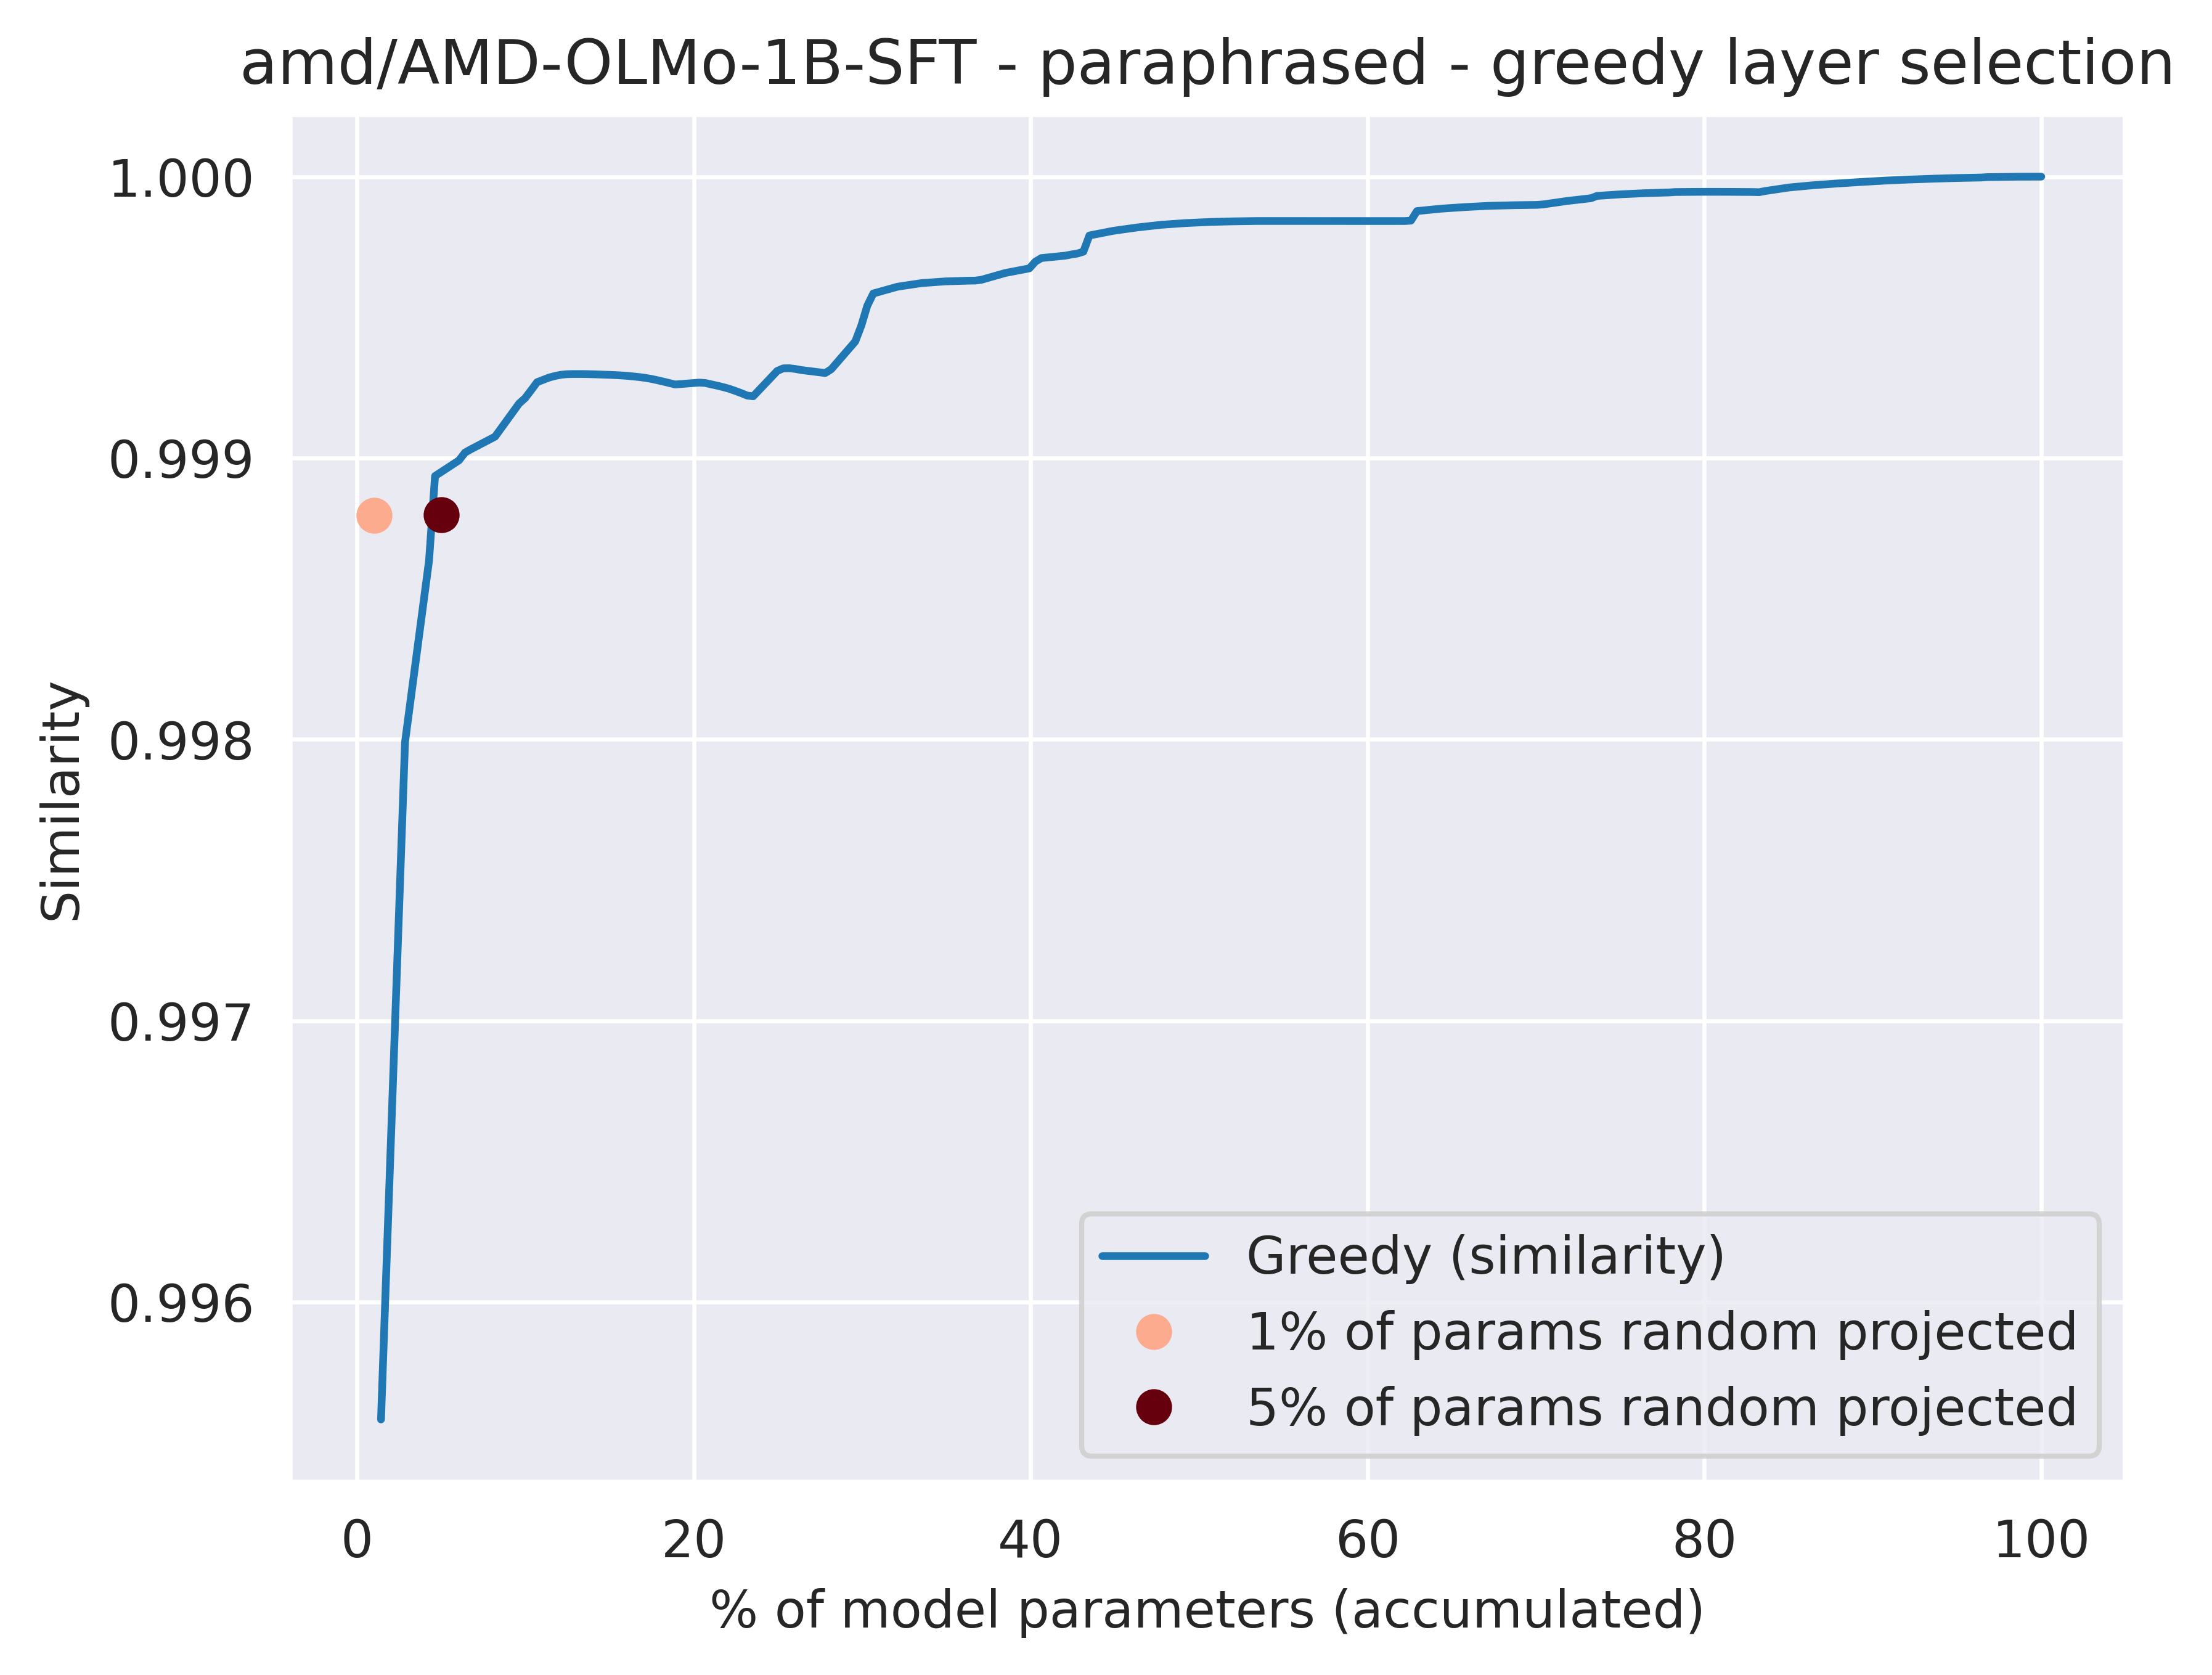
\includegraphics[width=\textwidth]{figures/results/paraphrased/greedy_layer_selection.png}
        \caption{Paraphrased}
        \label{fig:greedy_layer_selection_paraphrased}
    \end{subfigure}
    \hfill
    \begin{subfigure}[b]{0.49\textwidth}
        \centering
        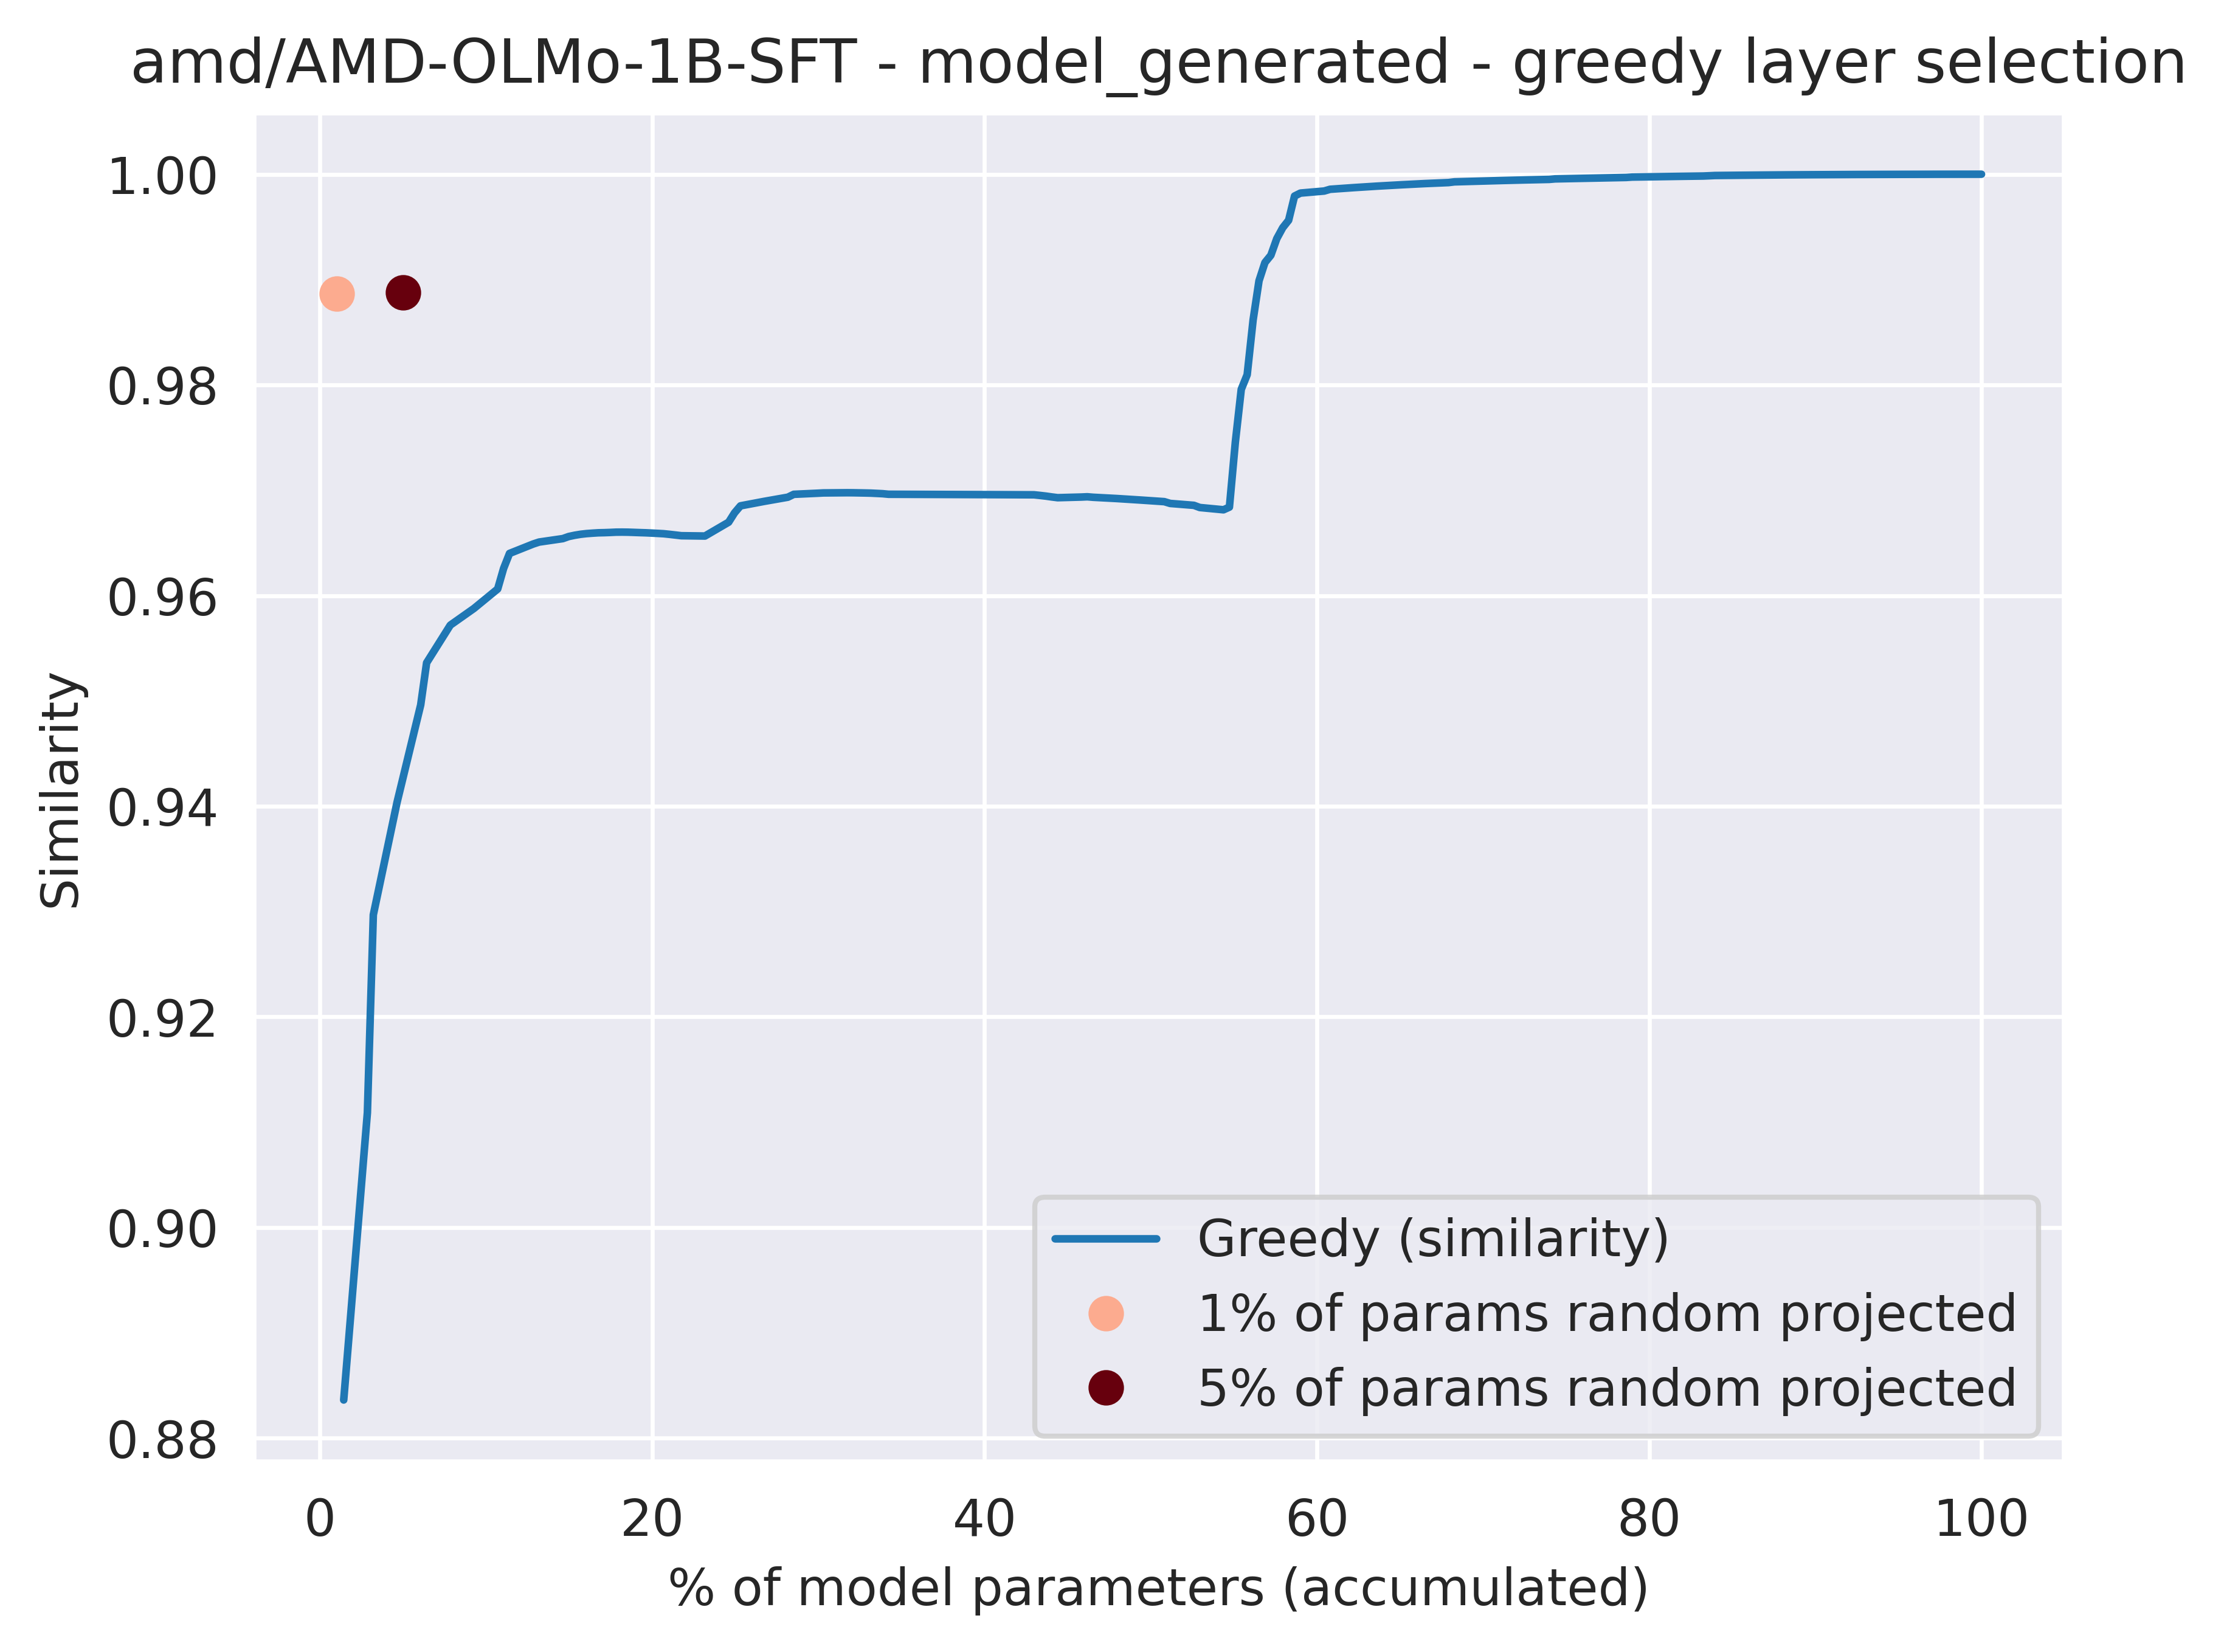
\includegraphics[width=\textwidth]{figures/results/model-generated/greedy_layer_selection.png}
        \caption{Model-generated}
        \label{fig:greedy_layer_selection_model_generated}
    \end{subfigure}
    \caption{Greedy Layer Selection compared to random projection by similarity to the full model gradient.}
    \label{fig:greedy_layer_selection}
\end{figure}


\section{Execution Time}\label{sec:exec_time}
Wall-clock times include dataset loading and all computations after model/tokenizer initialization. Each Slurm job logs its duration; totals are obtained by summing across jobs assigned to disjoint partitions. The report separates (i) computation of intermediate dot products (Section~\ref{subsec:intermediate_results}) and (ii) gradient-similarity evaluation with and without random projections.
\\\\
The execution time is measured after the model and the tokenizer is loaded. Hence, it contains the time to load the dataset from the disk and perform all computations. Each \emph{Slurm} job logs its execution time separately and saves it on disk for later inspections. To make the results comparable, the individual times from the jobs are summed. Table~\ref{tab:execution_times} shows the execution times on the hardware described above described in Section~\ref{sec:hardware}. In this context, \emph{dot-products} refers to the computation of the intermediate dot-products mentioned in Subsection~\ref{subsec:intermediate_results} and \emph{gradient similarity} refers to the calculation of cosine similarities for the gradients. 
\begin{table}[H]
    \centering
    \begin{tabular}{|l l|c|c|}
        \hline
        \textbf{Computation Type} & & \textbf{Paraphrased (h)} & \textbf{Model-generated (h)} \\
        \hline
        Dot-products & & 3.54 & 3.35 \\
        \hline
        \multirow{2}{*}{Gradient similarity} 
            & without RP & 4.05 & 5.39 \\
            & with RP & 927.48 & 925.63 \\
        \hline
    \end{tabular}
    \caption{Execution times (in hours) for dot-products and gradient similarity (with and without \acrfull{rp}) under paraphrased and model-generated settings.}
    \label{tab:execution_times}
\end{table}
